\documentclass{scrbook}
\usepackage[utf8]{inputenc}			% Zeichensatzkodierung
\usepackage[T1]{fontenc}
\usepackage{amsmath}				% Mathematischer Formelsatz AMS
\usepackage{amsfonts}
\usepackage{amssymb}
\usepackage{csquotes}
\usepackage{todonotes}				% Annotationen von ToDos in der PDF
\usepackage[english, main=ngerman]{babel} % Sprache, Silbentrennung etc.
\usepackage[backend=biber, style=ieee]{biblatex}	%Bibliographie
\addbibresource{literature/literature.bib}
\usepackage{algorithm}				% Algorithmen Umgebung mit Algorithmenverzeichnis
\usepackage{listings}				% Quelltext
\usepackage{graphicx}				% Einbinden von Bildern

\usepackage{fancyhdr}
\usepackage{color}					% Farben wenn es sein muß
\usepackage{hyperref}				% Klickbare Verweise und \autoref{label}
\usepackage{booktabs}				% "Schöne" Tabellen	

% Custom-Liste für Themenallokation
\usepackage{enumitem}
\newlist{thallok}{enumerate}{10}
\setlist[thallok]{label*=\arabic*.}

\begin{document}
	
	%
%	Hier werden Titel, Bearbeiter und das Datum eingetragen
%
%\newcommand\svthema{}
\newcommand\svperson{Jan Beier, Nils Dunker, Leonard Fricke, Niklas Haldorn, Kay Heider, \linebreak Jona Lukas Heinrichs, Mathieu Herkersdorf, Carsten Kellner, Markus Mügge, Thomas Rysch, Jannik Stadtler, Tom Voellmer}
\newcommand\svdatum{\today} % \today für das aktuelle Datum, sonst als Text eintragen
\newcommand\lvname{Projektgruppe: Entwicklung eines 3D RPG Videospiels mittels prozeduraler Inhaltsgenerieung und Deep Reinforcement Learning}
\newcommand\lvtyp{SS 2022 - WS 2022/2023}
\newcommand\lvinst{TU Dortmund}

%\hypersetup{ % Thema und Author in die Meta-Daten der PDF
%	pdftitle={Seminararbeit zum Thema: \svthema} 
%	pdfauthor={\svperson}
%}	


	
	% Hier wird der Titel-Bereich formatiert
	% Die zuvor definierten Textbausteine werden hier verwendet.
	\title{ \huge\textbf{Projektgruppe: \linebreak \linebreak Entwicklung eines 3D RPG Videospiels mittels prozeduraler Inhaltsgenerierung und Deep Reinforcement Learning} }
	\author{Jan Beier \and Nils Dunker \and Leonard Fricke \and Niklas Haldorn \and Kay Heider \and Jona Lukas Heinrichs \and Mathieu Herkersdorf \and Carsten Kellner \and Markus Mügge \and Thomas Rysch \and Jannik Stadtler \and Tom Voellmer}
	\date{\LARGE{\svdatum} \linebreak \linebreak \normalsize \centering 
\includegraphics[width=0.4\textwidth]{resources/img/tu-dortmund.png} \linebreak \linebreak \large\textsc{"`\lvname"'} \linebreak \linebreak \large{\lvtyp} · \large{\lvinst}}
	
	\maketitle
	\thispagestyle{empty} % lässt die Seitennummer auf der Titelseite verschwinden
	\pagenumbering{Roman}
	
	\cleardoublepage
	\tableofcontents			% Inhaltsverzeichnis ... nicht für kurze Dokumente!
	\cleardoublepage
	
	\chapter{Danksagungen}
% TODO Jemand sollte das mal irgendwo hinschieben, wo es hinsoll 
Die erforderlichen Berechnungen wurden auf dem Linux-HPC-Cluster der Technischen Universität Dortmund (LiDO3) durchgeführt, in Teilen durch die Forschungsgroßgeräte-Initiative der Deutschen Forschungsgemeinschaft (DFG) unter der Projektnummer 271512359 gefördert.

\chapter{Einleitung}

\section{Motivation und Problemstellung}

Die prozedurale Generierung von NPCs sowie das Erlernen von Bewegungen und das Animieren dieser stellt heutzutage in der Videospielindustrie eine zentrale Herausforderung dar. Nicht nur müssen Kreaturen effizient und somit oftmals zur Laufzeit generiert werden, sondern es müssen auch die Animationen welche durch maschinelles Lernen erlernt werden, auf ein möglichst breites Spektrum an Kreaturen anwendbar sein. Dabei ist es also essentiell, dass das Training der Kreaturen möglichst generalisiert stattfindet, sodass bei der Kreatur-Generierung eine große, sich bei den Körpermerkmalen variierende Menge der Kreaturen erzeugt werden kann, wodurch weniger Einschränkungen für die Körpereigenschaften der NPCs aufkommen. Somit sollten also die Animationen auf einen möglichst breiten Pool von Kreaturen anwendbar sein, ohne für zufällig erzeugte, potentiell neue, Körpermerkmale neu trainieren zu müssen.

Weiterhin muss bei der Generierung von Spielfiguren die relevante Herausforderung des automatischen Aufspannens eines Meshes über den bis zu diesem Zeitpunkt untexturierten Körper einer Kreatur gelöst werden; das sogenannte \textit{Automatic Rigging}, welches ebenfalls zu dem prozeduralen Erzeugen von Kreaturen dazugehört. Es muss also hier das relevante Problem betrachtet werden, Meshes welche ggf. ebenfalls prozedural erzeugt werden, auf das breite Spektrum von verschiedenen Körperausprägungen des Kreaturen-Pools anwenden zu können, ohne dass es zu sehr von den Körperformen der Kreaturen abweicht.

Ferner könnte die prozedurale Generierung von Inhalten in einem Videospiel nicht nur zum Erzeugen von Kreaturen zum Einsatz kommen, sondern auch für die Spielwelt selbst. % Damit könnte ... Notiz für Thomas: Sobald Inhalte von World-Generation stehen, hier ein wenig ausführen.



\section{Zielsetzung und Vorgehensweise}

\section{Übersicht}

Während der Projektgruppe haben sich ... Untergruppen/Teams für die jeweiligen Bereiche ... herausgestellt.

Zuerst werden in dem zweiten Kapitel (\ref{Grundlagen}) alle Grundlagen beschrieben in Bezug auf die angeführten Themenbereiche der Projektgruppe welche in der Seminarphase gegenseitig vorgestellt wurden (\ref{Zielsetzung_und_Vorgehensweise}). Basierend auf diesen Themengebieten werden dann in Kapitel \ref{Verwandte_Arbeiten} verwandte Arbeiten und Literatur vorgestellt, welche sowohl während der Evaluation in der Seminarphase erforscht wurden, als auch in der späteren Erarbeitung weiterer Themen und Algorithmen (Kapitel \ref{Fachliches_Vorgehen} und \ref{Technische_Umsetzung}) ausgemacht wurden. Sobald die Grundlagen über die Themen der späteren fachlichen und technischen Vorgehensweise geklärt sind, wird in Kapitel \ref{Fachliches_Vorgehen} das fachliche Vorgehen beschrieben, welches sich während der Entwicklungsphase der verschiedenen Bereiche (s. Kapitel \ref{Zielsetzung_und_Vorgehensweise}) erschlossen hat. Nachdem die fachbezogene Vorgehensweise bekannt ist, wird im Anschluss die Umsetzung in Kapitel \ref{Technische_Umsetzung} evaluiert, wie die in Kapitel \ref{Fachliches_Vorgehen} beschriebenen Verfahren und Algorithmen technisch umgesetzt sind. Anschließend werden in Kapitel \ref{Vorlaeufige_Ergebnisse} die (\textcolor{red}{Zwischen-})Ergebnisse präsentiert und diskutiert (\ref{Diskussion}), \textcolor{red}{hier später für den Endbericht ausführen wie genau und wodrauf bezogen die Ergebnisse diskutiert werden}. Schließlich wird in Kapitel \ref{Ausblick} zusammengefasst, auf welche (Forschungs-)Bereiche die Erkenntnisse dieser Studie ausgeweitet werden können. \textcolor{red}{Weiter ausführen?}
	
	\chapter{Grundlagen}
\label{Grundlagen}

(Die benutzten) Vortragsthemen vom Anfang hier als eigene Unterkapitel beschreiben.

% Generation
%  Grundlagen L-System: Allgemein, Theoretischer Hintergrund, 2D, 3D
\section{L-System}
Eine zentrale Eigenschaft in der Natur ist die Selbstähnlichkeit von Strukturen auf makroskopischer und mikroskopischer Ebene~\cite{Shaker2016}.
Das heißt, es lassen sich dieselben geometrischen Strukturen in verschiedenen Größenordnungen wiederfinden.
Beispielsweise ähneln die Knospen eines Blumenkohls auch seiner äußeren Struktur, wie in Abbildung~\ref{fig:Blumenkohl}\footnote{Quelle: \url{https://commons.wikimedia.org/wiki/File:Blumenkohl-1.jpg}, Autor: Rainer Zenz, CC BY-SA 3.0 \url{http://creativecommons.org/licenses/by-sa/3.0/}, via Wikimedia Commons} zu sehen ist.
\begin{figure}[ht]
    \centering
    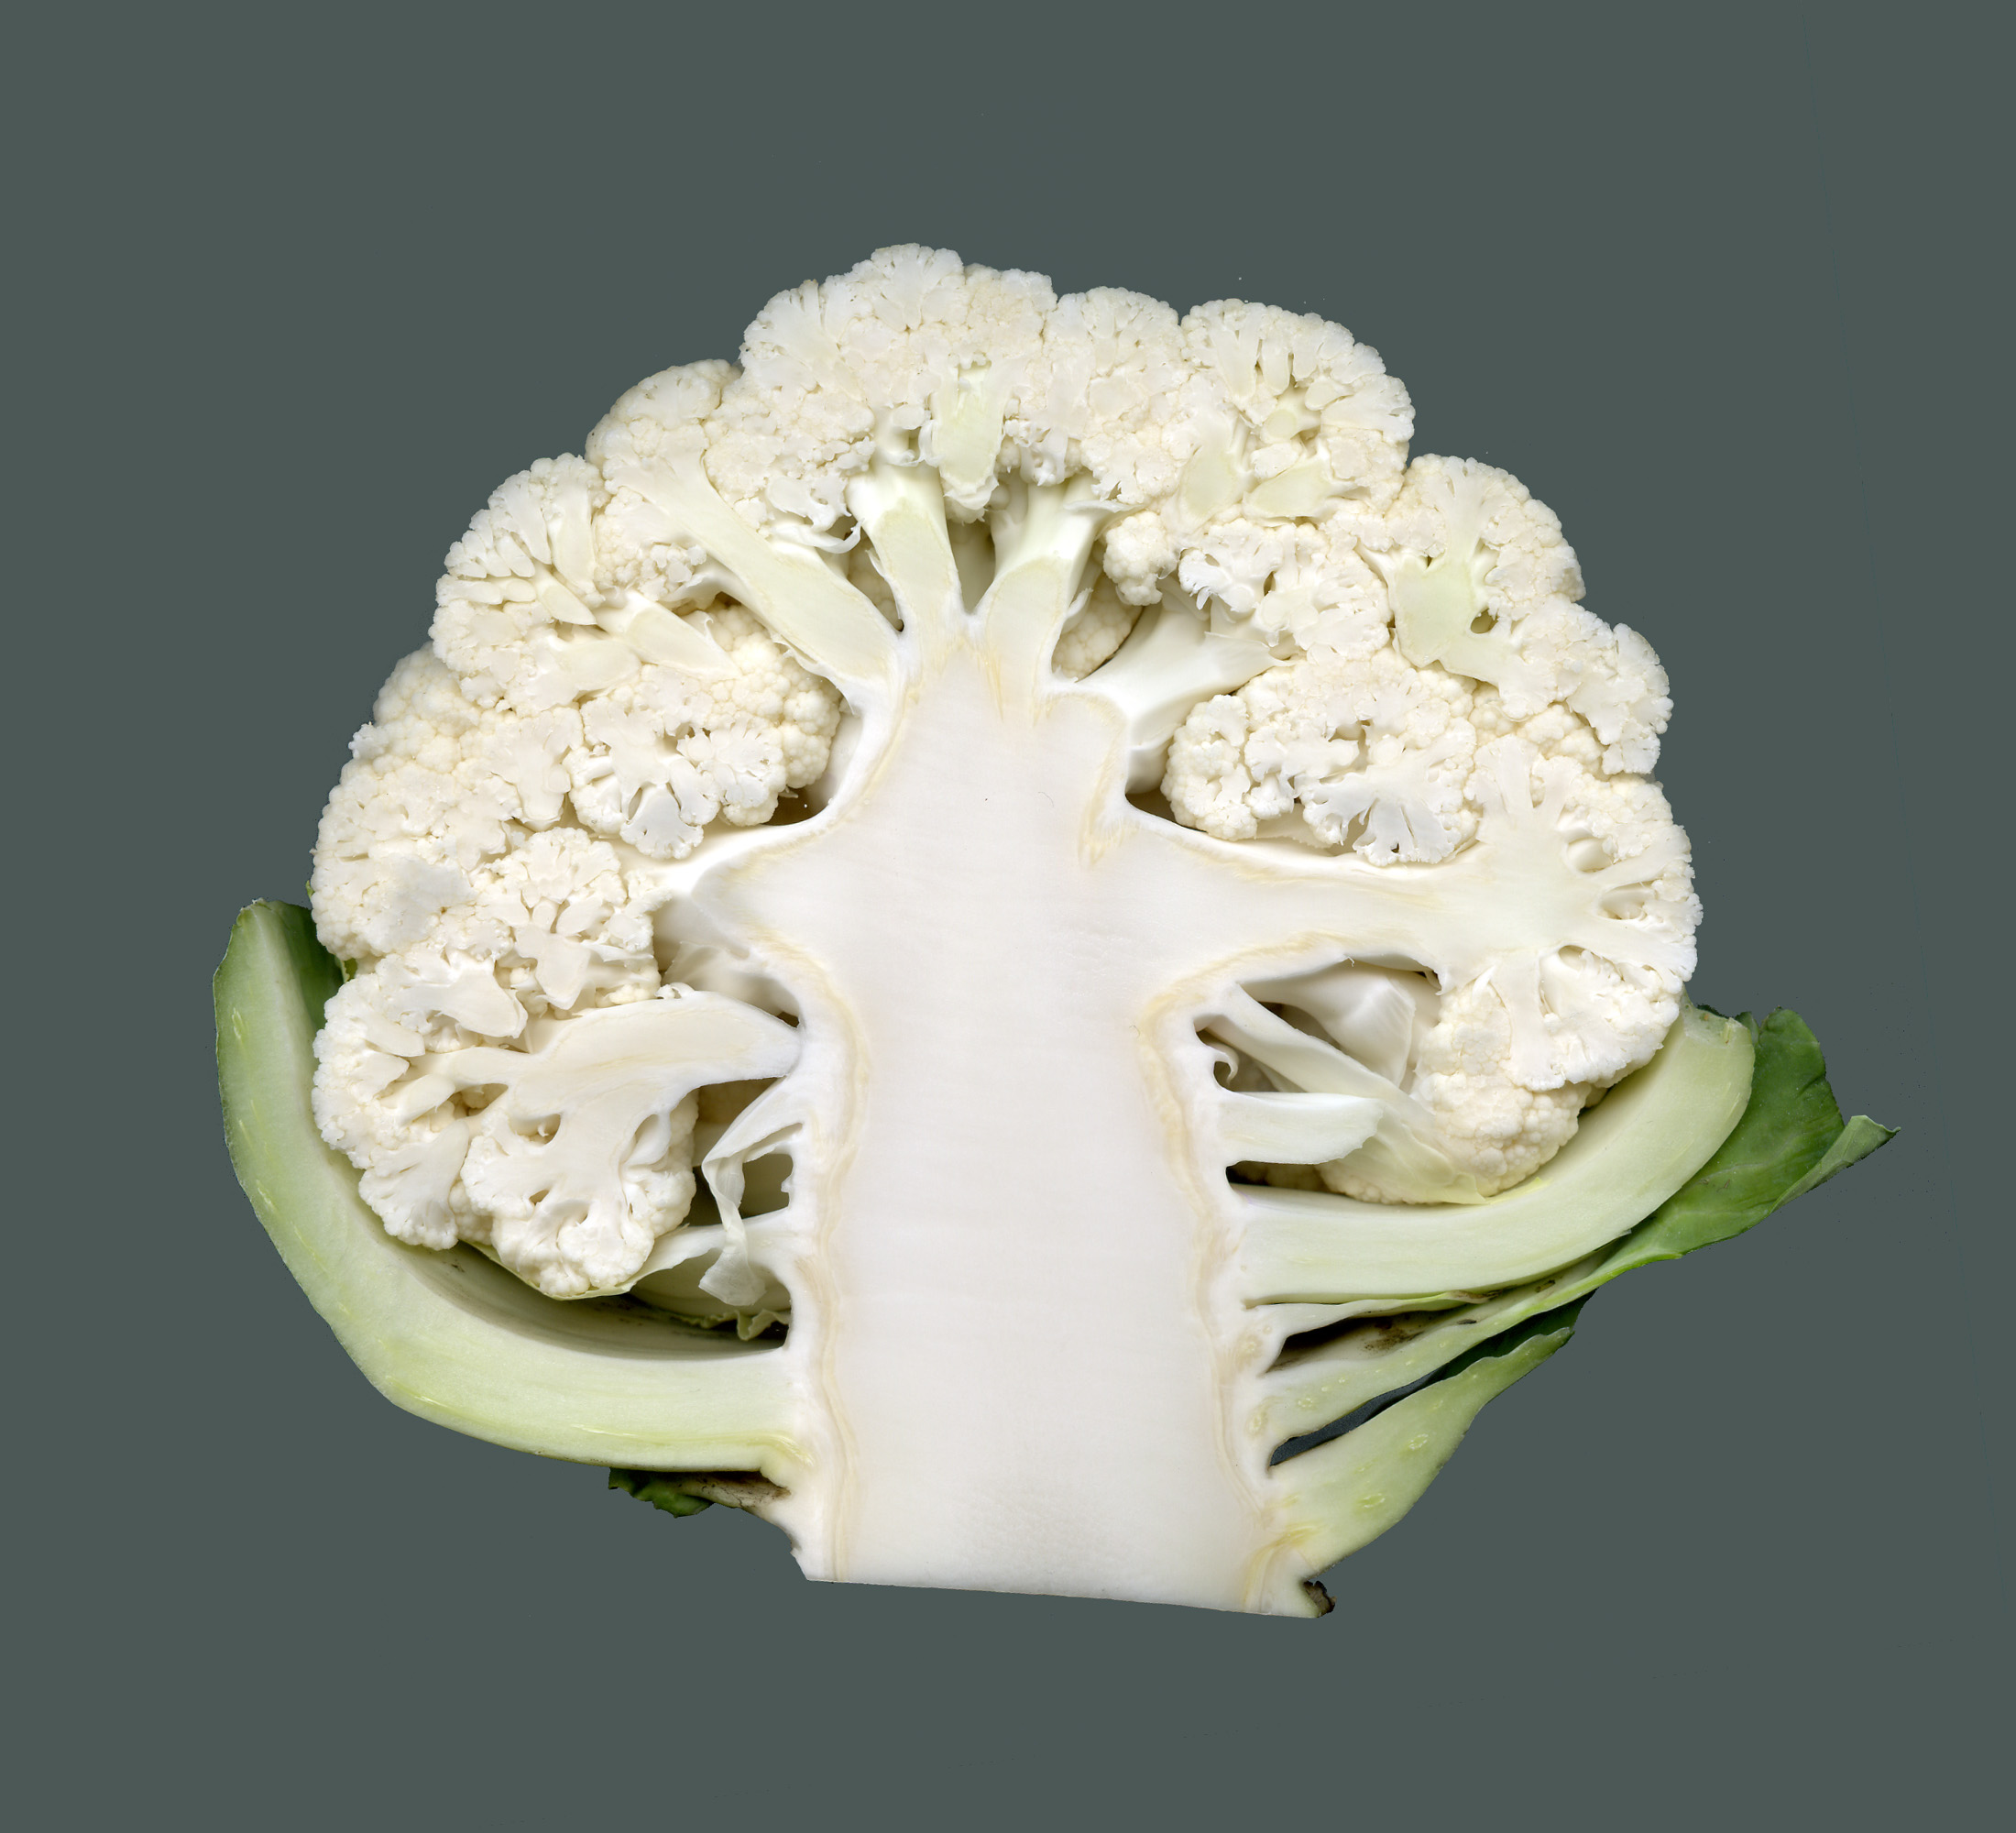
\includegraphics[width=0.5\linewidth]{chapters/02_Grundlagen/L_System/Blumenkohl-1.jpg}
    \caption{Blumenkohl}\label{fig:Blumenkohl}
\end{figure}

Um diese Eigenschaften präzise und strukturell darzustellen kann ein Lindenmayer-System (L-System)~\cite{lindenmayer1990} eingesetzt werden.
Die Basis eines L-Systems bildet eine kontextfreie Grammatik $G=(N,T,S,P)$ mit einer Menge von Nicht-Terminalsymbolen $N$, einer Menge von Terminalsymbolen $T$, einem Startsymbol $S$ und einer Menge von Produktionen $P$.
Der Unterschied zwischen einem L-System und einer üblichen kontextfreien Grammatik besteht darin, dass in einem Ableitungsschritt eines L-Systems parallel alle Nicht-Terminale ersetzt werden.
Zusätzlich werden nur eine feste Anzahl an Ableitungsschritten durchgeführt und es kann anstatt eines Startsymbols auch ein Startstring angegeben werden.

\subsection{Grafische Darstellung in 2D}
Der resultierende String einer Ableitung kann grafisch als Zeichenvorschriften für \emph{turtle graphics} interpretiert werden.
In \emph{turtle graphics} gibt es eine \emph{turtle}, oder Zeichenkopf, der initial in eine Richtung zeigt und sich in zwei oder drei Dimensionen fortbewegen kann.
Bei jeder Fortbewegung wird entlang der aktuellen Richtung der turtle und der hinterlegten Distanz, eine Strecke gezeichnet.
Die Symbole der Grammatik werden hierbei als Fortbewegung um eine gewisse Distanz oder eine Drehung interpretiert.
In Abbildung~\ref{fig:L-System 2D Rotation} ist eine Visualisierung dieses Konzeptes zu sehen.
Hier ist die turtle initial nach oben gerichtet.

\begin{figure}[ht]
    \centering
    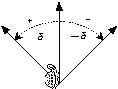
\includegraphics[width=0.5\linewidth]{chapters/02_Grundlagen/L_System/L_System_2D.pdf}
    \caption{L-System 2D Rotation}\label{fig:L-System 2D Rotation}
\end{figure}

Ohne Erweiterungen entstehen hierbei immer zusammenhängende Strukturen, die an einem Stück gezeichnet werden müssen; die turtle darf also nicht springen.
Das heißt, Blätter, Äste oder Stängel sind nur schwer zu realisieren.


\subsection{Erweiterungen}
Um komplexere Strukturen abzubilden, werden zusätzliche Symbole eingesetzt und die Auswertung erweitert.
Zwei übliche Erweiterung, die besonders zur Generierung von Vegetation nützlich sind, sind \emph{Bracketed L-Systeme} und \emph{Stochastische L-Systeme}.

\subsubsection{Bracketed L-Systeme}
\emph{Bracketed L-Systeme}~\cite*{Shaker2016} werden zur Definition von Strukturen eingesetzt, bei denen die turtle ihre Position ändern muss, ohne dass ein Strich gezeichnet wird.
Damit die generierte Struktur zusammenhängend bleibt, wird die Position und aktuelle Richtung der turtle auf einem Stack gespeichert und kann durch \texttt{push} und \texttt{pop} Operationen verwaltet werden.
Die turtle kann sich nur fortbewegen ohne zu zeichnen, indem sie an eine vorherige Position zurückspringt.
Die Menge der Terminalsymbole wird dabei um \texttt{[} für die \texttt{push} Operation und \texttt{]} für \texttt{pop} erweitert.
Bei dem Lesen eines \texttt{[}, wird die aktuelle Position und Rotation der turtle auf dem Stack gespeichert.
Wenn ein \texttt{]} gelesen wird, dann wird die turtle zu der Position und Rotation zurückgesetzt, die auf dem Stack als oberstes Element gespeichert worden war.

Mit dieser Erweiterung können insbesondere auch Äste von Bäumen oder Stängel von Blumen gezeichnet werden.
Ein Beispiel für eine Art von Strauch kann mittels dieses L-Systems erzeugt werden:
\begin{itemize}
    \item Nicht-Terminalsymbole $N=\{F\}$
    \item Terminalsymbole $T=\{\texttt{+},\texttt{-},\texttt{[},\texttt{]}\}$
    \item Startstring $S=F$
    \item Produktionen:
    \begin{align*}
        F\rightarrow~F\texttt{[+}F\texttt{]}F\texttt{[-}F\texttt{]}\texttt{[}F\texttt{]}
    \end{align*}
\end{itemize}

Hierbei beschreibt das Nicht-Terminalsymbol $F$ eine Fortbewegung, \texttt{+} und \texttt{-} jeweils eine Drehung um \ang{30} nach links bzw. rechts in 2D und \texttt{[}, \texttt{]} beschreiben die \texttt{push} und \texttt{pop} Operationen.
Für die ersten drei Ableitungsschritte sind die generierten Strukturen in Abbildung~\ref{fig:Bracketed} dargestellt.

\begin{figure}[ht]
    \begin{subfigure}[t]{.3\textwidth}
        \centering
        \resizebox{!}{100px}{\begin{tikzpicture}\draw (0,0) -- (0,0);
\draw (0,0) -- (0,10);
\draw (0,10) -- (-5,19);
\draw (0,10) -- (0,10);
\draw (0,10) -- (0,20);
\draw (0,20) -- (5,29);
\draw (0,20) -- (0,20);
\draw (0,20) -- (0,30);
\draw (0,20) -- (0,20);
\end{tikzpicture}}

        \caption*{Ein Ableitungsschritt}
    \end{subfigure}
    \hfill
    \begin{subfigure}[t]{.3\textwidth}
        \centering
        \resizebox{!}{100bp}{\begin{tikzpicture}\draw (0,0) -- (0,0);
\draw (0,0) -- (0,10);
\draw (0,10) -- (-5,19);
\draw (0,10) -- (0,10);
\draw (0,10) -- (0,20);
\draw (0,20) -- (5,29);
\draw (0,20) -- (0,20);
\draw (0,20) -- (0,30);
\draw (0,20) -- (0,20);
\draw (0,20) -- (-5,29);
\draw (-5,29) -- (-14,34);
\draw (-5,29) -- (-5,29);
\draw (-5,29) -- (-10,38);
\draw (-10,38) -- (-10,48);
\draw (-10,38) -- (-10,38);
\draw (-10,38) -- (-15,47);
\draw (-10,38) -- (-10,38);
\draw (0,20) -- (0,20);
\draw (0,20) -- (0,30);
\draw (0,30) -- (-5,39);
\draw (0,30) -- (0,30);
\draw (0,30) -- (0,40);
\draw (0,40) -- (5,49);
\draw (0,40) -- (0,40);
\draw (0,40) -- (0,50);
\draw (0,40) -- (0,40);
\draw (0,40) -- (5,49);
\draw (5,49) -- (5,59);
\draw (5,49) -- (5,49);
\draw (5,49) -- (10,58);
\draw (10,58) -- (19,63);
\draw (10,58) -- (10,58);
\draw (10,58) -- (15,67);
\draw (10,58) -- (10,58);
\draw (0,40) -- (0,40);
\draw (0,40) -- (0,50);
\draw (0,50) -- (-5,59);
\draw (0,50) -- (0,50);
\draw (0,50) -- (0,60);
\draw (0,60) -- (5,69);
\draw (0,60) -- (0,60);
\draw (0,60) -- (0,70);
\draw (0,60) -- (0,60);
\draw (0,40) -- (0,40);
\end{tikzpicture}}

        \caption*{Zwei Ableitungsschritte}
    \end{subfigure}
    \hfill
    \begin{subfigure}[t]{.3\textwidth}
        \centering
        \resizebox{!}{100px}{\begin{tikzpicture}\draw (0,0) -- (0,0);
\draw (0,0) -- (0,10);
\draw (0,10) -- (-5,19);
\draw (0,10) -- (0,10);
\draw (0,10) -- (0,20);
\draw (0,20) -- (5,29);
\draw (0,20) -- (0,20);
\draw (0,20) -- (0,30);
\draw (0,20) -- (0,20);
\draw (0,20) -- (-5,29);
\draw (-5,29) -- (-14,34);
\draw (-5,29) -- (-5,29);
\draw (-5,29) -- (-10,38);
\draw (-10,38) -- (-10,48);
\draw (-10,38) -- (-10,38);
\draw (-10,38) -- (-15,47);
\draw (-10,38) -- (-10,38);
\draw (0,20) -- (0,20);
\draw (0,20) -- (0,30);
\draw (0,30) -- (-5,39);
\draw (0,30) -- (0,30);
\draw (0,30) -- (0,40);
\draw (0,40) -- (5,49);
\draw (0,40) -- (0,40);
\draw (0,40) -- (0,50);
\draw (0,40) -- (0,40);
\draw (0,40) -- (5,49);
\draw (5,49) -- (5,59);
\draw (5,49) -- (5,49);
\draw (5,49) -- (10,58);
\draw (10,58) -- (19,63);
\draw (10,58) -- (10,58);
\draw (10,58) -- (15,67);
\draw (10,58) -- (10,58);
\draw (0,40) -- (0,40);
\draw (0,40) -- (0,50);
\draw (0,50) -- (-5,59);
\draw (0,50) -- (0,50);
\draw (0,50) -- (0,60);
\draw (0,60) -- (5,69);
\draw (0,60) -- (0,60);
\draw (0,60) -- (0,70);
\draw (0,60) -- (0,60);
\draw (0,40) -- (0,40);
\draw (0,40) -- (-5,49);
\draw (-5,49) -- (-14,54);
\draw (-5,49) -- (-5,49);
\draw (-5,49) -- (-10,58);
\draw (-10,58) -- (-10,68);
\draw (-10,58) -- (-10,58);
\draw (-10,58) -- (-15,67);
\draw (-10,58) -- (-10,58);
\draw (-10,58) -- (-19,63);
\draw (-19,63) -- (-29,63);
\draw (-19,63) -- (-19,63);
\draw (-19,63) -- (-28,68);
\draw (-28,68) -- (-33,77);
\draw (-28,68) -- (-28,68);
\draw (-28,68) -- (-37,73);
\draw (-28,68) -- (-28,68);
\draw (-10,58) -- (-10,58);
\draw (-10,58) -- (-15,67);
\draw (-15,67) -- (-24,72);
\draw (-15,67) -- (-15,67);
\draw (-15,67) -- (-20,76);
\draw (-20,76) -- (-20,86);
\draw (-20,76) -- (-20,76);
\draw (-20,76) -- (-25,85);
\draw (-20,76) -- (-20,76);
\draw (-20,76) -- (-20,86);
\draw (-20,86) -- (-25,95);
\draw (-20,86) -- (-20,86);
\draw (-20,86) -- (-20,96);
\draw (-20,96) -- (-15,105);
\draw (-20,96) -- (-20,96);
\draw (-20,96) -- (-20,106);
\draw (-20,96) -- (-20,96);
\draw (-20,76) -- (-20,76);
\draw (-20,76) -- (-25,85);
\draw (-25,85) -- (-34,90);
\draw (-25,85) -- (-25,85);
\draw (-25,85) -- (-30,94);
\draw (-30,94) -- (-30,104);
\draw (-30,94) -- (-30,94);
\draw (-30,94) -- (-35,103);
\draw (-30,94) -- (-30,94);
\draw (-20,76) -- (-20,76);
\draw (0,40) -- (0,40);
\draw (0,40) -- (0,50);
\draw (0,50) -- (-5,59);
\draw (0,50) -- (0,50);
\draw (0,50) -- (0,60);
\draw (0,60) -- (5,69);
\draw (0,60) -- (0,60);
\draw (0,60) -- (0,70);
\draw (0,60) -- (0,60);
\draw (0,60) -- (-5,69);
\draw (-5,69) -- (-14,74);
\draw (-5,69) -- (-5,69);
\draw (-5,69) -- (-10,78);
\draw (-10,78) -- (-10,88);
\draw (-10,78) -- (-10,78);
\draw (-10,78) -- (-15,87);
\draw (-10,78) -- (-10,78);
\draw (0,60) -- (0,60);
\draw (0,60) -- (0,70);
\draw (0,70) -- (-5,79);
\draw (0,70) -- (0,70);
\draw (0,70) -- (0,80);
\draw (0,80) -- (5,89);
\draw (0,80) -- (0,80);
\draw (0,80) -- (0,90);
\draw (0,80) -- (0,80);
\draw (0,80) -- (5,89);
\draw (5,89) -- (5,99);
\draw (5,89) -- (5,89);
\draw (5,89) -- (10,98);
\draw (10,98) -- (19,103);
\draw (10,98) -- (10,98);
\draw (10,98) -- (15,107);
\draw (10,98) -- (10,98);
\draw (0,80) -- (0,80);
\draw (0,80) -- (0,90);
\draw (0,90) -- (-5,99);
\draw (0,90) -- (0,90);
\draw (0,90) -- (0,100);
\draw (0,100) -- (5,109);
\draw (0,100) -- (0,100);
\draw (0,100) -- (0,110);
\draw (0,100) -- (0,100);
\draw (0,80) -- (0,80);
\draw (0,80) -- (5,89);
\draw (5,89) -- (5,99);
\draw (5,89) -- (5,89);
\draw (5,89) -- (10,98);
\draw (10,98) -- (19,103);
\draw (10,98) -- (10,98);
\draw (10,98) -- (15,107);
\draw (10,98) -- (10,98);
\draw (10,98) -- (10,108);
\draw (10,108) -- (5,117);
\draw (10,108) -- (10,108);
\draw (10,108) -- (10,118);
\draw (10,118) -- (15,127);
\draw (10,118) -- (10,118);
\draw (10,118) -- (10,128);
\draw (10,118) -- (10,118);
\draw (10,98) -- (10,98);
\draw (10,98) -- (15,107);
\draw (15,107) -- (15,117);
\draw (15,107) -- (15,107);
\draw (15,107) -- (20,116);
\draw (20,116) -- (29,121);
\draw (20,116) -- (20,116);
\draw (20,116) -- (25,125);
\draw (20,116) -- (20,116);
\draw (20,116) -- (29,121);
\draw (29,121) -- (34,130);
\draw (29,121) -- (29,121);
\draw (29,121) -- (38,126);
\draw (38,126) -- (48,126);
\draw (38,126) -- (38,126);
\draw (38,126) -- (47,131);
\draw (38,126) -- (38,126);
\draw (20,116) -- (20,116);
\draw (20,116) -- (25,125);
\draw (25,125) -- (25,135);
\draw (25,125) -- (25,125);
\draw (25,125) -- (30,134);
\draw (30,134) -- (39,139);
\draw (30,134) -- (30,134);
\draw (30,134) -- (35,143);
\draw (30,134) -- (30,134);
\draw (20,116) -- (20,116);
\draw (0,80) -- (0,80);
\draw (0,80) -- (0,90);
\draw (0,90) -- (-5,99);
\draw (0,90) -- (0,90);
\draw (0,90) -- (0,100);
\draw (0,100) -- (5,109);
\draw (0,100) -- (0,100);
\draw (0,100) -- (0,110);
\draw (0,100) -- (0,100);
\draw (0,100) -- (-5,109);
\draw (-5,109) -- (-14,114);
\draw (-5,109) -- (-5,109);
\draw (-5,109) -- (-10,118);
\draw (-10,118) -- (-10,128);
\draw (-10,118) -- (-10,118);
\draw (-10,118) -- (-15,127);
\draw (-10,118) -- (-10,118);
\draw (0,100) -- (0,100);
\draw (0,100) -- (0,110);
\draw (0,110) -- (-5,119);
\draw (0,110) -- (0,110);
\draw (0,110) -- (0,120);
\draw (0,120) -- (5,129);
\draw (0,120) -- (0,120);
\draw (0,120) -- (0,130);
\draw (0,120) -- (0,120);
\draw (0,120) -- (5,129);
\draw (5,129) -- (5,139);
\draw (5,129) -- (5,129);
\draw (5,129) -- (10,138);
\draw (10,138) -- (19,143);
\draw (10,138) -- (10,138);
\draw (10,138) -- (15,147);
\draw (10,138) -- (10,138);
\draw (0,120) -- (0,120);
\draw (0,120) -- (0,130);
\draw (0,130) -- (-5,139);
\draw (0,130) -- (0,130);
\draw (0,130) -- (0,140);
\draw (0,140) -- (5,149);
\draw (0,140) -- (0,140);
\draw (0,140) -- (0,150);
\draw (0,140) -- (0,140);
\draw (0,120) -- (0,120);
\draw (0,80) -- (0,80);
\end{tikzpicture}}

        \caption*{Drei Ableitungsschritte}
    \end{subfigure}
    \caption{Darstellung der ersten drei Ableitungsschritte eines Bracketed L-Systems}\label{fig:Bracketed}
\end{figure}


\subsubsection{Stochastische L-Systeme}
Eine Eigenschaft von den bisher verwendeten L-Systemen ist, dass die Produktionen deterministisch ausgewertet werden und die resultierenden Strings eindeutig sind.
Um realistische Pflanzen generieren zu können muss jedoch etwas Variation eingeführt werden; es wäre also vorteilhaft, wenn die Produktionen nicht-deterministisch ausgewertet werden.
Dazu kann ein \emph{stochastisches L-System}~\cite*{Shaker2016} verwendet werden.
Hierbei kann es mehrere Produktionen mit gleichen linken Seiten geben.
Jeweils über die Menge von Produktionen mit gleicher linken Seite wird eine Wahrscheinlichkeitsverteilung erstellt.
Das heißt die Auswahl der Ersetzung eines Nicht-Terminalsymbols erfolgt zufällig.

Im Folgenden ist ein Beispiel für ein stochastisches Bracketed L-System gegeben:
\begin{itemize}
    \item Nicht-Terminalsymbole $N=\{F\}$
    \item Terminalsymbole $T=\{\texttt{+},\texttt{-},\texttt{[},\texttt{]}\}$
    \item Startstring $S=F$
    \item Produktionen:
    \begin{align*}
        F\xrightarrow{0.33} & ~F\texttt{[+}F\texttt{]}F\texttt{[-}F\texttt{]} F \\
        F\xrightarrow{0.33} & ~F\texttt{[+}F\texttt{]} F                         \\
        F\xrightarrow{0.34} & ~F\texttt{[-}F\texttt{]} F
    \end{align*}
\end{itemize}

Hier gibt es für das Nicht-Terminal $F$ drei Produktionen, zwei Produktionen werden mit einer Wahrscheinlichkeit von \SI{33}{\percent} gewählt und eine Produktion wird mit \SI{34}{\percent} gewählt.
Drei resultierende Bilder dieses L-Systems sind in Abbildung~\ref{fig:Stochastic} gegeben.
Es ist gut erkennbar wie aus einem L-System deutlich unterschiedliche Strukturen generiert werden können, die jedoch alle ähnliche Grundstrukturen aufweisen.
\begin{figure}[ht]
    \begin{subfigure}[t]{.25\textwidth}
        \centering
        \resizebox{!}{175px}{\begin{tikzpicture}\draw (0,0) -- (0,0);
\draw (0,0) -- (0,10);
\draw (0,10) -- (-5,19);
\draw (0,10) -- (0,10);
\draw (0,10) -- (0,20);
\draw (0,20) -- (5,29);
\draw (5,29) -- (5,39);
\draw (5,29) -- (5,29);
\draw (5,29) -- (10,38);
\draw (0,20) -- (0,20);
\draw (0,20) -- (0,30);
\draw (0,30) -- (-5,39);
\draw (0,30) -- (0,30);
\draw (0,30) -- (0,40);
\draw (0,40) -- (5,49);
\draw (5,49) -- (14,54);
\draw (5,49) -- (5,49);
\draw (5,49) -- (10,58);
\draw (10,58) -- (10,68);
\draw (10,68) -- (5,77);
\draw (10,68) -- (10,68);
\draw (10,68) -- (10,78);
\draw (10,58) -- (10,58);
\draw (10,58) -- (15,67);
\draw (15,67) -- (15,77);
\draw (15,67) -- (15,67);
\draw (15,67) -- (20,76);
\draw (0,40) -- (0,40);
\draw (0,40) -- (0,50);
\draw (0,50) -- (5,59);
\draw (0,50) -- (0,50);
\draw (0,50) -- (0,60);
\draw (0,60) -- (-5,69);
\draw (0,60) -- (0,60);
\draw (0,60) -- (0,70);
\draw (0,70) -- (5,79);
\draw (5,79) -- (5,89);
\draw (5,79) -- (5,79);
\draw (5,79) -- (10,88);
\draw (0,70) -- (0,70);
\draw (0,70) -- (0,80);
\draw (0,80) -- (5,89);
\draw (0,80) -- (0,80);
\draw (0,80) -- (0,90);
\draw (0,90) -- (-5,99);
\draw (0,90) -- (0,90);
\draw (0,90) -- (0,100);
\draw (0,100) -- (-5,109);
\draw (-5,109) -- (-5,119);
\draw (-5,109) -- (-5,109);
\draw (-5,109) -- (-10,118);
\draw (-10,118) -- (-19,123);
\draw (-10,118) -- (-10,118);
\draw (-10,118) -- (-15,127);
\draw (-15,127) -- (-15,137);
\draw (-15,137) -- (-10,146);
\draw (-15,137) -- (-15,137);
\draw (-15,137) -- (-15,147);
\draw (-15,127) -- (-15,127);
\draw (-15,127) -- (-20,136);
\draw (-20,136) -- (-20,146);
\draw (-20,136) -- (-20,136);
\draw (-20,136) -- (-25,145);
\draw (-25,145) -- (-34,150);
\draw (-34,150) -- (-44,150);
\draw (-34,150) -- (-34,150);
\draw (-34,150) -- (-43,155);
\draw (-25,145) -- (-25,145);
\draw (-25,145) -- (-30,154);
\draw (-30,154) -- (-30,164);
\draw (-30,154) -- (-30,154);
\draw (-30,154) -- (-35,163);
\draw (-35,163) -- (-44,168);
\draw (-35,163) -- (-35,163);
\draw (-35,163) -- (-40,172);
\draw (0,100) -- (0,100);
\draw (0,100) -- (0,110);
\draw (0,110) -- (-5,119);
\draw (0,110) -- (0,110);
\draw (0,110) -- (0,120);
\draw (0,120) -- (-5,129);
\draw (-5,129) -- (-5,139);
\draw (-5,129) -- (-5,129);
\draw (-5,129) -- (-10,138);
\draw (-10,138) -- (-19,143);
\draw (-10,138) -- (-10,138);
\draw (-10,138) -- (-15,147);
\draw (0,120) -- (0,120);
\draw (0,120) -- (0,130);
\draw (0,130) -- (5,139);
\draw (0,130) -- (0,130);
\draw (0,130) -- (0,140);
\draw (0,140) -- (-5,149);
\draw (0,140) -- (0,140);
\draw (0,140) -- (0,150);
\draw (0,150) -- (5,159);
\draw (5,159) -- (14,164);
\draw (5,159) -- (5,159);
\draw (5,159) -- (10,168);
\draw (10,168) -- (10,178);
\draw (10,168) -- (10,168);
\draw (10,168) -- (15,177);
\draw (15,177) -- (24,182);
\draw (24,182) -- (29,191);
\draw (24,182) -- (24,182);
\draw (24,182) -- (33,187);
\draw (15,177) -- (15,177);
\draw (15,177) -- (20,186);
\draw (20,186) -- (29,191);
\draw (20,186) -- (20,186);
\draw (20,186) -- (25,195);
\draw (25,195) -- (25,205);
\draw (25,205) -- (30,214);
\draw (25,205) -- (25,205);
\draw (25,205) -- (25,215);
\draw (25,215) -- (20,224);
\draw (25,215) -- (25,215);
\draw (25,215) -- (25,225);
\draw (25,225) -- (30,234);
\draw (30,234) -- (39,239);
\draw (30,234) -- (30,234);
\draw (30,234) -- (35,243);
\draw (35,243) -- (35,253);
\draw (35,243) -- (35,243);
\draw (35,243) -- (40,252);
\draw (25,225) -- (25,225);
\draw (25,225) -- (25,235);
\draw (25,235) -- (20,244);
\draw (25,235) -- (25,235);
\draw (25,235) -- (25,245);
\draw (25,245) -- (20,254);
\draw (20,254) -- (20,264);
\draw (20,254) -- (20,254);
\draw (20,254) -- (15,263);
\draw (25,245) -- (25,245);
\draw (25,245) -- (25,255);
\draw (25,255) -- (30,264);
\draw (25,255) -- (25,255);
\draw (25,255) -- (25,265);
\draw (25,265) -- (20,274);
\draw (25,265) -- (25,265);
\draw (25,265) -- (25,275);
\draw (25,195) -- (25,195);
\draw (25,195) -- (30,204);
\draw (30,204) -- (30,214);
\draw (30,204) -- (30,204);
\draw (30,204) -- (35,213);
\draw (35,213) -- (35,223);
\draw (35,223) -- (30,232);
\draw (35,223) -- (35,223);
\draw (35,223) -- (35,233);
\draw (35,213) -- (35,213);
\draw (35,213) -- (40,222);
\draw (40,222) -- (49,227);
\draw (40,222) -- (40,222);
\draw (40,222) -- (45,231);
\draw (45,231) -- (45,241);
\draw (45,231) -- (45,231);
\draw (45,231) -- (50,240);
\draw (0,150) -- (0,150);
\draw (0,150) -- (0,160);
\draw (0,160) -- (-5,169);
\draw (0,160) -- (0,160);
\draw (0,160) -- (0,170);
\draw (0,170) -- (5,179);
\draw (5,179) -- (14,184);
\draw (5,179) -- (5,179);
\draw (5,179) -- (10,188);
\draw (10,188) -- (10,198);
\draw (10,188) -- (10,188);
\draw (10,188) -- (15,197);
\draw (0,170) -- (0,170);
\draw (0,170) -- (0,180);
\draw (0,180) -- (-5,189);
\draw (0,180) -- (0,180);
\draw (0,180) -- (0,190);
\draw (0,190) -- (5,199);
\draw (5,199) -- (14,204);
\draw (5,199) -- (5,199);
\draw (5,199) -- (10,208);
\draw (10,208) -- (10,218);
\draw (10,208) -- (10,208);
\draw (10,208) -- (15,217);
\draw (15,217) -- (24,222);
\draw (24,222) -- (29,231);
\draw (24,222) -- (24,222);
\draw (24,222) -- (33,227);
\draw (15,217) -- (15,217);
\draw (15,217) -- (20,226);
\draw (20,226) -- (29,231);
\draw (20,226) -- (20,226);
\draw (20,226) -- (25,235);
\draw (25,235) -- (25,245);
\draw (25,245) -- (30,254);
\draw (25,245) -- (25,245);
\draw (25,245) -- (25,255);
\draw (25,235) -- (25,235);
\draw (25,235) -- (30,244);
\draw (30,244) -- (39,249);
\draw (30,244) -- (30,244);
\draw (30,244) -- (35,253);
\draw (0,190) -- (0,190);
\draw (0,190) -- (0,200);
\draw (0,200) -- (5,209);
\draw (0,200) -- (0,200);
\draw (0,200) -- (0,210);
\draw (0,210) -- (-5,219);
\draw (0,210) -- (0,210);
\draw (0,210) -- (0,220);
\draw (0,220) -- (5,229);
\draw (5,229) -- (14,234);
\draw (5,229) -- (5,229);
\draw (5,229) -- (10,238);
\draw (0,220) -- (0,220);
\draw (0,220) -- (0,230);
\draw (0,230) -- (5,239);
\draw (0,230) -- (0,230);
\draw (0,230) -- (0,240);
\draw (0,240) -- (-5,249);
\draw (0,240) -- (0,240);
\draw (0,240) -- (0,250);
\draw (0,250) -- (-5,259);
\draw (-5,259) -- (-14,264);
\draw (-5,259) -- (-5,259);
\draw (-5,259) -- (-10,268);
\draw (-10,268) -- (-19,273);
\draw (-19,273) -- (-24,282);
\draw (-19,273) -- (-19,273);
\draw (-19,273) -- (-28,278);
\draw (-10,268) -- (-10,268);
\draw (-10,268) -- (-15,277);
\draw (-15,277) -- (-15,287);
\draw (-15,277) -- (-15,277);
\draw (-15,277) -- (-20,286);
\draw (-20,286) -- (-29,291);
\draw (-20,286) -- (-20,286);
\draw (-20,286) -- (-25,295);
\draw (-25,295) -- (-25,305);
\draw (-25,305) -- (-20,314);
\draw (-25,305) -- (-25,305);
\draw (-25,305) -- (-25,315);
\draw (-25,315) -- (-30,324);
\draw (-25,315) -- (-25,315);
\draw (-25,315) -- (-25,325);
\draw (-25,325) -- (-30,334);
\draw (-30,334) -- (-30,344);
\draw (-30,334) -- (-30,334);
\draw (-30,334) -- (-35,343);
\draw (-25,325) -- (-25,325);
\draw (-25,325) -- (-25,335);
\draw (-25,335) -- (-30,344);
\draw (-25,335) -- (-25,335);
\draw (-25,335) -- (-25,345);
\draw (-25,295) -- (-25,295);
\draw (-25,295) -- (-30,304);
\draw (-30,304) -- (-30,314);
\draw (-30,304) -- (-30,304);
\draw (-30,304) -- (-35,313);
\draw (-35,313) -- (-44,318);
\draw (-35,313) -- (-35,313);
\draw (-35,313) -- (-40,322);
\draw (-40,322) -- (-40,332);
\draw (-40,332) -- (-35,341);
\draw (-40,332) -- (-40,332);
\draw (-40,332) -- (-40,342);
\draw (-40,322) -- (-40,322);
\draw (-40,322) -- (-45,331);
\draw (-45,331) -- (-45,341);
\draw (-45,331) -- (-45,331);
\draw (-45,331) -- (-50,340);
\draw (-50,340) -- (-59,345);
\draw (-50,340) -- (-50,340);
\draw (-50,340) -- (-55,349);
\draw (-55,349) -- (-64,354);
\draw (-64,354) -- (-69,363);
\draw (-64,354) -- (-64,354);
\draw (-64,354) -- (-73,359);
\draw (-73,359) -- (-83,359);
\draw (-73,359) -- (-73,359);
\draw (-73,359) -- (-82,364);
\draw (-55,349) -- (-55,349);
\draw (-55,349) -- (-60,358);
\draw (-60,358) -- (-69,363);
\draw (-60,358) -- (-60,358);
\draw (-60,358) -- (-65,367);
\draw (0,250) -- (0,250);
\draw (0,250) -- (0,260);
\draw (0,260) -- (5,269);
\draw (0,260) -- (0,260);
\draw (0,260) -- (0,270);
\draw (0,270) -- (-5,279);
\draw (-5,279) -- (-5,289);
\draw (-5,279) -- (-5,279);
\draw (-5,279) -- (-10,288);
\draw (0,270) -- (0,270);
\draw (0,270) -- (0,280);
\draw (0,280) -- (5,289);
\draw (0,280) -- (0,280);
\draw (0,280) -- (0,290);
\draw (0,290) -- (-5,299);
\draw (0,290) -- (0,290);
\draw (0,290) -- (0,300);
\draw (0,300) -- (5,309);
\draw (5,309) -- (5,319);
\draw (5,309) -- (5,309);
\draw (5,309) -- (10,318);
\draw (10,318) -- (19,323);
\draw (19,323) -- (24,332);
\draw (19,323) -- (19,323);
\draw (19,323) -- (28,328);
\draw (10,318) -- (10,318);
\draw (10,318) -- (15,327);
\draw (15,327) -- (15,337);
\draw (15,327) -- (15,327);
\draw (15,327) -- (20,336);
\draw (20,336) -- (20,346);
\draw (20,346) -- (15,355);
\draw (20,346) -- (20,346);
\draw (20,346) -- (20,356);
\draw (20,336) -- (20,336);
\draw (20,336) -- (25,345);
\draw (25,345) -- (34,350);
\draw (25,345) -- (25,345);
\draw (25,345) -- (30,354);
\draw (30,354) -- (30,364);
\draw (30,354) -- (30,354);
\draw (30,354) -- (35,363);
\draw (0,300) -- (0,300);
\draw (0,300) -- (0,310);
\draw (0,310) -- (-5,319);
\draw (0,310) -- (0,310);
\draw (0,310) -- (0,320);
\draw (0,320) -- (5,329);
\draw (5,329) -- (14,334);
\draw (5,329) -- (5,329);
\draw (5,329) -- (10,338);
\draw (10,338) -- (10,348);
\draw (10,338) -- (10,338);
\draw (10,338) -- (15,347);
\draw (0,320) -- (0,320);
\draw (0,320) -- (0,330);
\draw (0,330) -- (5,339);
\draw (0,330) -- (0,330);
\draw (0,330) -- (0,340);
\draw (0,340) -- (-5,349);
\draw (-5,349) -- (-14,354);
\draw (-5,349) -- (-5,349);
\draw (-5,349) -- (-10,358);
\draw (-10,358) -- (-10,368);
\draw (-10,368) -- (-5,377);
\draw (-10,368) -- (-10,368);
\draw (-10,368) -- (-10,378);
\draw (-10,358) -- (-10,358);
\draw (-10,358) -- (-15,367);
\draw (-15,367) -- (-15,377);
\draw (-15,367) -- (-15,367);
\draw (-15,367) -- (-20,376);
\draw (-20,376) -- (-29,381);
\draw (-20,376) -- (-20,376);
\draw (-20,376) -- (-25,385);
\draw (0,340) -- (0,340);
\draw (0,340) -- (0,350);
\draw (0,350) -- (-5,359);
\draw (0,350) -- (0,350);
\draw (0,350) -- (0,360);
\draw (0,360) -- (5,369);
\draw (5,369) -- (14,374);
\draw (5,369) -- (5,369);
\draw (5,369) -- (10,378);
\draw (0,360) -- (0,360);
\draw (0,360) -- (0,370);
\draw (0,370) -- (-5,379);
\draw (0,370) -- (0,370);
\draw (0,370) -- (0,380);
\draw (0,380) -- (-5,389);
\draw (-5,389) -- (-14,394);
\draw (-5,389) -- (-5,389);
\draw (-5,389) -- (-10,398);
\draw (0,380) -- (0,380);
\draw (0,380) -- (0,390);
\draw (0,390) -- (5,399);
\draw (0,390) -- (0,390);
\draw (0,390) -- (0,400);
\draw (0,400) -- (-5,409);
\draw (0,400) -- (0,400);
\draw (0,400) -- (0,410);
\end{tikzpicture}}

    \end{subfigure}
    \hfill
    \begin{subfigure}[t]{.25\textwidth}
        \centering
        \resizebox{!}{175bp}{\begin{tikzpicture}\draw (0,0) -- (0,0);
\draw (0,0) -- (0,10);
\draw (0,10) -- (5,19);
\draw (0,10) -- (0,10);
\draw (0,10) -- (0,20);
\draw (0,20) -- (5,29);
\draw (5,29) -- (5,39);
\draw (5,29) -- (5,29);
\draw (5,29) -- (10,38);
\draw (0,20) -- (0,20);
\draw (0,20) -- (0,30);
\draw (0,30) -- (5,39);
\draw (0,30) -- (0,30);
\draw (0,30) -- (0,40);
\draw (0,40) -- (-5,49);
\draw (0,40) -- (0,40);
\draw (0,40) -- (0,50);
\draw (0,50) -- (-5,59);
\draw (-5,59) -- (-5,69);
\draw (-5,59) -- (-5,59);
\draw (-5,59) -- (-10,68);
\draw (-10,68) -- (-19,73);
\draw (-10,68) -- (-10,68);
\draw (-10,68) -- (-15,77);
\draw (0,50) -- (0,50);
\draw (0,50) -- (0,60);
\draw (0,60) -- (5,69);
\draw (0,60) -- (0,60);
\draw (0,60) -- (0,70);
\draw (0,70) -- (-5,79);
\draw (-5,79) -- (-14,84);
\draw (-5,79) -- (-5,79);
\draw (-5,79) -- (-10,88);
\draw (-10,88) -- (-10,98);
\draw (-10,98) -- (-15,107);
\draw (-10,98) -- (-10,98);
\draw (-10,98) -- (-10,108);
\draw (-10,88) -- (-10,88);
\draw (-10,88) -- (-15,97);
\draw (-15,97) -- (-24,102);
\draw (-15,97) -- (-15,97);
\draw (-15,97) -- (-20,106);
\draw (-20,106) -- (-29,111);
\draw (-29,111) -- (-39,111);
\draw (-29,111) -- (-29,111);
\draw (-29,111) -- (-38,116);
\draw (-20,106) -- (-20,106);
\draw (-20,106) -- (-25,115);
\draw (-25,115) -- (-34,120);
\draw (-25,115) -- (-25,115);
\draw (-25,115) -- (-30,124);
\draw (0,70) -- (0,70);
\draw (0,70) -- (0,80);
\draw (0,80) -- (5,89);
\draw (0,80) -- (0,80);
\draw (0,80) -- (0,90);
\draw (0,90) -- (-5,99);
\draw (0,90) -- (0,90);
\draw (0,90) -- (0,100);
\draw (0,100) -- (5,109);
\draw (5,109) -- (5,119);
\draw (5,109) -- (5,109);
\draw (5,109) -- (10,118);
\draw (0,100) -- (0,100);
\draw (0,100) -- (0,110);
\draw (0,110) -- (-5,119);
\draw (0,110) -- (0,110);
\draw (0,110) -- (0,120);
\draw (0,120) -- (-5,129);
\draw (-5,129) -- (-5,139);
\draw (-5,129) -- (-5,129);
\draw (-5,129) -- (-10,138);
\draw (-10,138) -- (-19,143);
\draw (-10,138) -- (-10,138);
\draw (-10,138) -- (-15,147);
\draw (-15,147) -- (-15,157);
\draw (-15,157) -- (-10,166);
\draw (-15,157) -- (-15,157);
\draw (-15,157) -- (-15,167);
\draw (-15,147) -- (-15,147);
\draw (-15,147) -- (-20,156);
\draw (-20,156) -- (-20,166);
\draw (-20,156) -- (-20,156);
\draw (-20,156) -- (-25,165);
\draw (-25,165) -- (-34,170);
\draw (-25,165) -- (-25,165);
\draw (-25,165) -- (-30,174);
\draw (-30,174) -- (-30,184);
\draw (-30,184) -- (-25,193);
\draw (-30,184) -- (-30,184);
\draw (-30,184) -- (-30,194);
\draw (-30,194) -- (-25,203);
\draw (-25,203) -- (-25,213);
\draw (-25,203) -- (-25,203);
\draw (-25,203) -- (-20,212);
\draw (-30,194) -- (-30,194);
\draw (-30,194) -- (-30,204);
\draw (-30,204) -- (-25,213);
\draw (-30,204) -- (-30,204);
\draw (-30,204) -- (-30,214);
\draw (-30,214) -- (-35,223);
\draw (-35,223) -- (-35,233);
\draw (-35,223) -- (-35,223);
\draw (-35,223) -- (-40,232);
\draw (-40,232) -- (-49,237);
\draw (-40,232) -- (-40,232);
\draw (-40,232) -- (-45,241);
\draw (-30,214) -- (-30,214);
\draw (-30,214) -- (-30,224);
\draw (-30,224) -- (-25,233);
\draw (-30,224) -- (-30,224);
\draw (-30,224) -- (-30,234);
\draw (-30,234) -- (-35,243);
\draw (-30,234) -- (-30,234);
\draw (-30,234) -- (-30,244);
\draw (-30,174) -- (-30,174);
\draw (-30,174) -- (-35,183);
\draw (-35,183) -- (-35,193);
\draw (-35,183) -- (-35,183);
\draw (-35,183) -- (-40,192);
\draw (-40,192) -- (-49,197);
\draw (-40,192) -- (-40,192);
\draw (-40,192) -- (-45,201);
\draw (-45,201) -- (-54,206);
\draw (-54,206) -- (-64,206);
\draw (-54,206) -- (-54,206);
\draw (-54,206) -- (-63,211);
\draw (-45,201) -- (-45,201);
\draw (-45,201) -- (-50,210);
\draw (-50,210) -- (-50,220);
\draw (-50,210) -- (-50,210);
\draw (-50,210) -- (-55,219);
\draw (-55,219) -- (-64,224);
\draw (-55,219) -- (-55,219);
\draw (-55,219) -- (-60,228);
\draw (-60,228) -- (-69,233);
\draw (-69,233) -- (-79,233);
\draw (-69,233) -- (-69,233);
\draw (-69,233) -- (-78,238);
\draw (-78,238) -- (-83,247);
\draw (-83,247) -- (-83,257);
\draw (-83,247) -- (-83,247);
\draw (-83,247) -- (-88,256);
\draw (-78,238) -- (-78,238);
\draw (-78,238) -- (-87,243);
\draw (-87,243) -- (-97,243);
\draw (-87,243) -- (-87,243);
\draw (-87,243) -- (-96,248);
\draw (-60,228) -- (-60,228);
\draw (-60,228) -- (-65,237);
\draw (-65,237) -- (-74,242);
\draw (-65,237) -- (-65,237);
\draw (-65,237) -- (-70,246);
\draw (-70,246) -- (-70,256);
\draw (-70,256) -- (-65,265);
\draw (-70,256) -- (-70,256);
\draw (-70,256) -- (-70,266);
\draw (-70,246) -- (-70,246);
\draw (-70,246) -- (-75,255);
\draw (-75,255) -- (-84,260);
\draw (-75,255) -- (-75,255);
\draw (-75,255) -- (-80,264);
\draw (-80,264) -- (-89,269);
\draw (-89,269) -- (-94,278);
\draw (-89,269) -- (-89,269);
\draw (-89,269) -- (-98,274);
\draw (-98,274) -- (-108,274);
\draw (-98,274) -- (-98,274);
\draw (-98,274) -- (-107,279);
\draw (-80,264) -- (-80,264);
\draw (-80,264) -- (-85,273);
\draw (-85,273) -- (-85,283);
\draw (-85,273) -- (-85,273);
\draw (-85,273) -- (-90,282);
\draw (-90,282) -- (-99,287);
\draw (-90,282) -- (-90,282);
\draw (-90,282) -- (-95,291);
\draw (0,120) -- (0,120);
\draw (0,120) -- (0,130);
\draw (0,130) -- (5,139);
\draw (0,130) -- (0,130);
\draw (0,130) -- (0,140);
\draw (0,140) -- (-5,149);
\draw (0,140) -- (0,140);
\draw (0,140) -- (0,150);
\draw (0,150) -- (-5,159);
\draw (-5,159) -- (-14,164);
\draw (-5,159) -- (-5,159);
\draw (-5,159) -- (-10,168);
\draw (0,150) -- (0,150);
\draw (0,150) -- (0,160);
\draw (0,160) -- (5,169);
\draw (0,160) -- (0,160);
\draw (0,160) -- (0,170);
\draw (0,170) -- (-5,179);
\draw (-5,179) -- (-5,189);
\draw (-5,179) -- (-5,179);
\draw (-5,179) -- (-10,188);
\draw (-10,188) -- (-19,193);
\draw (-10,188) -- (-10,188);
\draw (-10,188) -- (-15,197);
\draw (-15,197) -- (-15,207);
\draw (-15,207) -- (-20,216);
\draw (-15,207) -- (-15,207);
\draw (-15,207) -- (-15,217);
\draw (-15,197) -- (-15,197);
\draw (-15,197) -- (-20,206);
\draw (-20,206) -- (-29,211);
\draw (-20,206) -- (-20,206);
\draw (-20,206) -- (-25,215);
\draw (0,170) -- (0,170);
\draw (0,170) -- (0,180);
\draw (0,180) -- (-5,189);
\draw (0,180) -- (0,180);
\draw (0,180) -- (0,190);
\draw (0,190) -- (-5,199);
\draw (-5,199) -- (-5,209);
\draw (-5,199) -- (-5,199);
\draw (-5,199) -- (-10,208);
\draw (0,190) -- (0,190);
\draw (0,190) -- (0,200);
\draw (0,200) -- (5,209);
\draw (0,200) -- (0,200);
\draw (0,200) -- (0,210);
\draw (0,210) -- (-5,219);
\draw (0,210) -- (0,210);
\draw (0,210) -- (0,220);
\end{tikzpicture}}

    \end{subfigure}
    \hfill
    \begin{subfigure}[t]{.25\textwidth}
        \centering
        \resizebox{!}{175px}{\begin{tikzpicture}\draw (0,0) -- (0,0);
\draw (0,0) -- (0,10);
\draw (0,10) -- (5,19);
\draw (0,10) -- (0,10);
\draw (0,10) -- (0,20);
\draw (0,20) -- (-5,29);
\draw (0,20) -- (0,20);
\draw (0,20) -- (0,30);
\draw (0,30) -- (-5,39);
\draw (-5,39) -- (-14,44);
\draw (-5,39) -- (-5,39);
\draw (-5,39) -- (-10,48);
\draw (0,30) -- (0,30);
\draw (0,30) -- (0,40);
\draw (0,40) -- (-5,49);
\draw (0,40) -- (0,40);
\draw (0,40) -- (0,50);
\draw (0,50) -- (-5,59);
\draw (-5,59) -- (-5,69);
\draw (-5,59) -- (-5,59);
\draw (-5,59) -- (-10,68);
\draw (-10,68) -- (-19,73);
\draw (-19,73) -- (-29,73);
\draw (-19,73) -- (-19,73);
\draw (-19,73) -- (-28,78);
\draw (-10,68) -- (-10,68);
\draw (-10,68) -- (-15,77);
\draw (-15,77) -- (-15,87);
\draw (-15,77) -- (-15,77);
\draw (-15,77) -- (-20,86);
\draw (-20,86) -- (-29,91);
\draw (-20,86) -- (-20,86);
\draw (-20,86) -- (-25,95);
\draw (0,50) -- (0,50);
\draw (0,50) -- (0,60);
\draw (0,60) -- (5,69);
\draw (0,60) -- (0,60);
\draw (0,60) -- (0,70);
\draw (0,70) -- (-5,79);
\draw (0,70) -- (0,70);
\draw (0,70) -- (0,80);
\draw (0,80) -- (5,89);
\draw (5,89) -- (14,94);
\draw (5,89) -- (5,89);
\draw (5,89) -- (10,98);
\draw (0,80) -- (0,80);
\draw (0,80) -- (0,90);
\draw (0,90) -- (-5,99);
\draw (0,90) -- (0,90);
\draw (0,90) -- (0,100);
\draw (0,100) -- (-5,109);
\draw (-5,109) -- (-5,119);
\draw (-5,109) -- (-5,109);
\draw (-5,109) -- (-10,118);
\draw (0,100) -- (0,100);
\draw (0,100) -- (0,110);
\draw (0,110) -- (5,119);
\draw (0,110) -- (0,110);
\draw (0,110) -- (0,120);
\draw (0,120) -- (-5,129);
\draw (0,120) -- (0,120);
\draw (0,120) -- (0,130);
\draw (0,130) -- (5,139);
\draw (5,139) -- (5,149);
\draw (5,139) -- (5,139);
\draw (5,139) -- (10,148);
\draw (10,148) -- (19,153);
\draw (19,153) -- (24,162);
\draw (19,153) -- (19,153);
\draw (19,153) -- (28,158);
\draw (10,148) -- (10,148);
\draw (10,148) -- (15,157);
\draw (15,157) -- (24,162);
\draw (15,157) -- (15,157);
\draw (15,157) -- (20,166);
\draw (20,166) -- (20,176);
\draw (20,166) -- (20,166);
\draw (20,166) -- (25,175);
\draw (25,175) -- (34,180);
\draw (34,180) -- (44,180);
\draw (34,180) -- (34,180);
\draw (34,180) -- (43,185);
\draw (43,185) -- (48,194);
\draw (43,185) -- (43,185);
\draw (43,185) -- (52,190);
\draw (52,190) -- (57,199);
\draw (57,199) -- (66,204);
\draw (57,199) -- (57,199);
\draw (57,199) -- (62,208);
\draw (62,208) -- (62,218);
\draw (62,208) -- (62,208);
\draw (62,208) -- (67,217);
\draw (52,190) -- (52,190);
\draw (52,190) -- (61,195);
\draw (61,195) -- (66,204);
\draw (61,195) -- (61,195);
\draw (61,195) -- (70,200);
\draw (25,175) -- (25,175);
\draw (25,175) -- (30,184);
\draw (30,184) -- (30,194);
\draw (30,184) -- (30,184);
\draw (30,184) -- (35,193);
\draw (35,193) -- (35,203);
\draw (35,203) -- (40,212);
\draw (35,203) -- (35,203);
\draw (35,203) -- (35,213);
\draw (35,193) -- (35,193);
\draw (35,193) -- (40,202);
\draw (40,202) -- (40,212);
\draw (40,202) -- (40,202);
\draw (40,202) -- (45,211);
\draw (0,130) -- (0,130);
\draw (0,130) -- (0,140);
\draw (0,140) -- (5,149);
\draw (0,140) -- (0,140);
\draw (0,140) -- (0,150);
\draw (0,150) -- (-5,159);
\draw (-5,159) -- (-5,169);
\draw (-5,159) -- (-5,159);
\draw (-5,159) -- (-10,168);
\draw (-10,168) -- (-19,173);
\draw (-10,168) -- (-10,168);
\draw (-10,168) -- (-15,177);
\draw (0,150) -- (0,150);
\draw (0,150) -- (0,160);
\draw (0,160) -- (-5,169);
\draw (0,160) -- (0,160);
\draw (0,160) -- (0,170);
\draw (0,170) -- (5,179);
\draw (5,179) -- (5,189);
\draw (5,179) -- (5,179);
\draw (5,179) -- (10,188);
\draw (10,188) -- (19,193);
\draw (19,193) -- (29,193);
\draw (19,193) -- (19,193);
\draw (19,193) -- (28,198);
\draw (28,198) -- (33,207);
\draw (28,198) -- (28,198);
\draw (28,198) -- (37,203);
\draw (10,188) -- (10,188);
\draw (10,188) -- (15,197);
\draw (15,197) -- (24,202);
\draw (15,197) -- (15,197);
\draw (15,197) -- (20,206);
\draw (20,206) -- (20,216);
\draw (20,206) -- (20,206);
\draw (20,206) -- (25,215);
\draw (25,215) -- (25,225);
\draw (25,225) -- (20,234);
\draw (25,225) -- (25,225);
\draw (25,225) -- (25,235);
\draw (25,215) -- (25,215);
\draw (25,215) -- (30,224);
\draw (30,224) -- (39,229);
\draw (30,224) -- (30,224);
\draw (30,224) -- (35,233);
\draw (0,170) -- (0,170);
\draw (0,170) -- (0,180);
\draw (0,180) -- (5,189);
\draw (0,180) -- (0,180);
\draw (0,180) -- (0,190);
\draw (0,190) -- (5,199);
\draw (5,199) -- (14,204);
\draw (5,199) -- (5,199);
\draw (5,199) -- (10,208);
\draw (10,208) -- (10,218);
\draw (10,208) -- (10,208);
\draw (10,208) -- (15,217);
\draw (0,190) -- (0,190);
\draw (0,190) -- (0,200);
\draw (0,200) -- (5,209);
\draw (0,200) -- (0,200);
\draw (0,200) -- (0,210);
\draw (0,210) -- (-5,219);
\draw (-5,219) -- (-5,229);
\draw (-5,219) -- (-5,219);
\draw (-5,219) -- (-10,228);
\draw (-10,228) -- (-19,233);
\draw (-10,228) -- (-10,228);
\draw (-10,228) -- (-15,237);
\draw (-15,237) -- (-15,247);
\draw (-15,247) -- (-10,256);
\draw (-15,247) -- (-15,247);
\draw (-15,247) -- (-15,257);
\draw (-15,237) -- (-15,237);
\draw (-15,237) -- (-20,246);
\draw (-20,246) -- (-20,256);
\draw (-20,246) -- (-20,246);
\draw (-20,246) -- (-25,255);
\draw (-25,255) -- (-34,260);
\draw (-34,260) -- (-44,260);
\draw (-34,260) -- (-34,260);
\draw (-34,260) -- (-43,265);
\draw (-25,255) -- (-25,255);
\draw (-25,255) -- (-30,264);
\draw (-30,264) -- (-39,269);
\draw (-30,264) -- (-30,264);
\draw (-30,264) -- (-35,273);
\draw (-35,273) -- (-44,278);
\draw (-44,278) -- (-49,287);
\draw (-44,278) -- (-44,278);
\draw (-44,278) -- (-53,283);
\draw (-53,283) -- (-63,283);
\draw (-53,283) -- (-53,283);
\draw (-53,283) -- (-62,288);
\draw (-62,288) -- (-67,297);
\draw (-67,297) -- (-76,302);
\draw (-67,297) -- (-67,297);
\draw (-67,297) -- (-72,306);
\draw (-62,288) -- (-62,288);
\draw (-62,288) -- (-71,293);
\draw (-71,293) -- (-76,302);
\draw (-71,293) -- (-71,293);
\draw (-71,293) -- (-80,298);
\draw (-80,298) -- (-90,298);
\draw (-80,298) -- (-80,298);
\draw (-80,298) -- (-89,303);
\draw (-35,273) -- (-35,273);
\draw (-35,273) -- (-40,282);
\draw (-40,282) -- (-40,292);
\draw (-40,282) -- (-40,282);
\draw (-40,282) -- (-45,291);
\draw (-45,291) -- (-45,301);
\draw (-45,301) -- (-40,310);
\draw (-45,301) -- (-45,301);
\draw (-45,301) -- (-45,311);
\draw (-45,311) -- (-50,320);
\draw (-45,311) -- (-45,311);
\draw (-45,311) -- (-45,321);
\draw (-45,291) -- (-45,291);
\draw (-45,291) -- (-50,300);
\draw (-50,300) -- (-59,305);
\draw (-50,300) -- (-50,300);
\draw (-50,300) -- (-55,309);
\draw (-55,309) -- (-64,314);
\draw (-64,314) -- (-69,323);
\draw (-64,314) -- (-64,314);
\draw (-64,314) -- (-73,319);
\draw (-55,309) -- (-55,309);
\draw (-55,309) -- (-60,318);
\draw (-60,318) -- (-60,328);
\draw (-60,318) -- (-60,318);
\draw (-60,318) -- (-65,327);
\draw (0,210) -- (0,210);
\draw (0,210) -- (0,220);
\draw (0,220) -- (5,229);
\draw (0,220) -- (0,220);
\draw (0,220) -- (0,230);
\draw (0,230) -- (-5,239);
\draw (-5,239) -- (-5,249);
\draw (-5,239) -- (-5,239);
\draw (-5,239) -- (-10,248);
\draw (-10,248) -- (-19,253);
\draw (-10,248) -- (-10,248);
\draw (-10,248) -- (-15,257);
\draw (0,230) -- (0,230);
\draw (0,230) -- (0,240);
\draw (0,240) -- (5,249);
\draw (0,240) -- (0,240);
\draw (0,240) -- (0,250);
\draw (0,250) -- (-5,259);
\draw (0,250) -- (0,250);
\draw (0,250) -- (0,260);
\draw (0,260) -- (-5,269);
\draw (-5,269) -- (-5,279);
\draw (-5,269) -- (-5,269);
\draw (-5,269) -- (-10,278);
\draw (-10,278) -- (-10,288);
\draw (-10,288) -- (-5,297);
\draw (-10,288) -- (-10,288);
\draw (-10,288) -- (-10,298);
\draw (-10,278) -- (-10,278);
\draw (-10,278) -- (-15,287);
\draw (-15,287) -- (-15,297);
\draw (-15,287) -- (-15,287);
\draw (-15,287) -- (-20,296);
\draw (-20,296) -- (-29,301);
\draw (-29,301) -- (-39,301);
\draw (-29,301) -- (-29,301);
\draw (-29,301) -- (-38,306);
\draw (-20,296) -- (-20,296);
\draw (-20,296) -- (-25,305);
\draw (-25,305) -- (-25,315);
\draw (-25,305) -- (-25,305);
\draw (-25,305) -- (-30,314);
\draw (-30,314) -- (-39,319);
\draw (-30,314) -- (-30,314);
\draw (-30,314) -- (-35,323);
\draw (0,260) -- (0,260);
\draw (0,260) -- (0,270);
\draw (0,270) -- (-5,279);
\draw (0,270) -- (0,270);
\draw (0,270) -- (0,280);
\draw (0,280) -- (5,289);
\draw (5,289) -- (14,294);
\draw (5,289) -- (5,289);
\draw (5,289) -- (10,298);
\draw (0,280) -- (0,280);
\draw (0,280) -- (0,290);
\draw (0,290) -- (5,299);
\draw (0,290) -- (0,290);
\draw (0,290) -- (0,300);
\end{tikzpicture}}

    \end{subfigure}
    \caption{Drei Resultate desselben stochastischen L-Systems}\label{fig:Stochastic}
\end{figure}


\subsubsection{Erweiterung in 3D}\label{subsub: L-System 3D}
Die L-Systeme aus den vorherigen Abschnitten haben stets zweidimensionale Strukturen erstellt.
Dabei wurden die Symbole \texttt{+} und \texttt{-} genutzt um die aktuelle Richtung der turtle in der Ebene zu rotieren.
Für Strukturen in drei Dimensionen kann diese Idee weiterverwendet werden.
Hierbei werden jeweils zwei Symbole für Rotationen um jede der drei Achsen eingeführt.
Die Symbole \texttt{+} und \texttt{-} rotieren die turtle um die $z$-Achse, \texttt{\&} und \texttt{\textasciicircum} rotieren um die $x$-Achse und \texttt{/} und \texttt{\textbackslash} rotieren um die $y$-Achse.

Ein Beispiel\footnote{L-System adaptiert von: \url{https://www.sidefx.com/docs/houdini/nodes/sop/lsystem.html#3d}} für ein L-System, das einen dreidimensionalen Baum erzeugt ist im Folgenden gegeben:
\begin{itemize}
    \item Nicht-Terminalsymbole $N=\{F\}$
    \item Terminalsymbole $T=\{\texttt{+},\texttt{-},\texttt{\&},\texttt{\textasciicircum},\texttt{/},\texttt{\textbackslash},\texttt{[},\texttt{]}\}$
    \item Startstring $S=FFFA$
    \item Produktionen:
    \begin{align*}
        A\rightarrow &~\texttt{[}B\texttt{]////[}B\texttt{]////}B \\
        B\rightarrow &~\texttt{\&}FFFA
    \end{align*}
\end{itemize}

Mit diesem L-System kann ein dreidimensionaler Baum wie in Abbildung~\ref{fig:L-System 3D Unity} in Unity erzeugt werden.
Es wurden 7 Ableitungsschritte durchgeführt und es wurde jeweils \ang{28} um die Achsen rotiert.

\begin{figure}[ht]
    \centering
    % \resizebox{\linewidth-3cm}{!}{%
        
    % }
    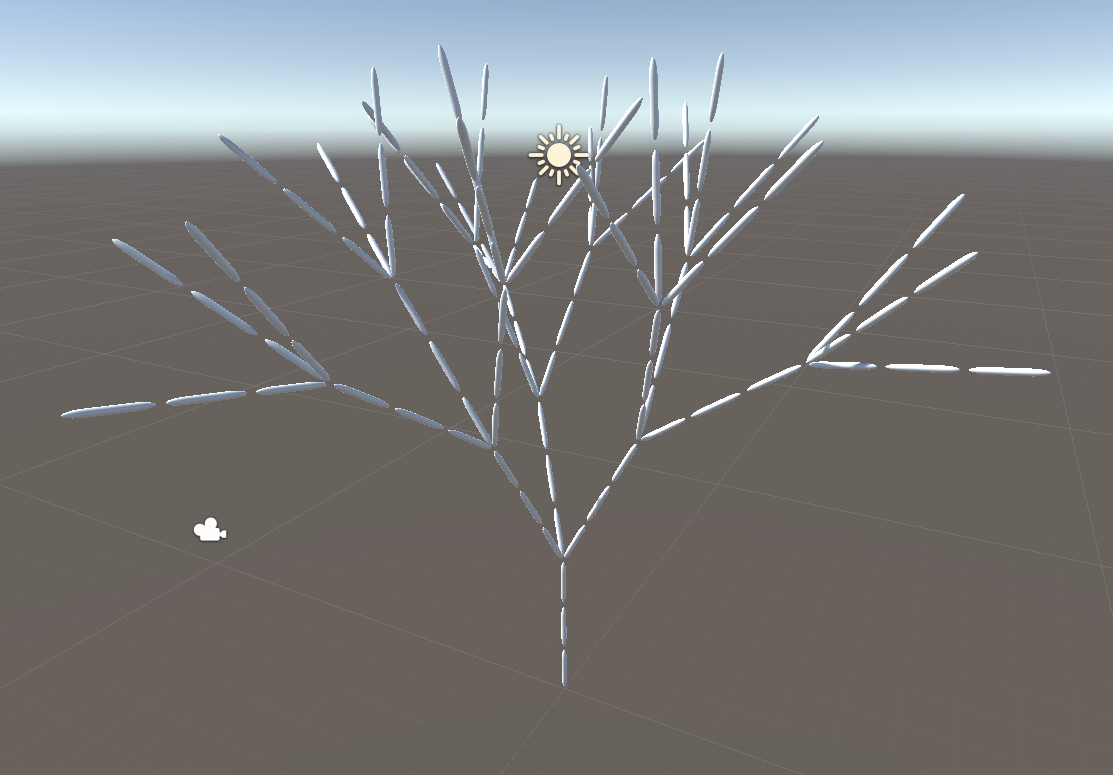
\includegraphics[width=0.5\linewidth]{chapters/02_Grundlagen/L_System/L_System_3D_Tree.png}
    \caption{L-System 3D Baum}\label{fig:L-System 3D Unity}
\end{figure}


\subsection{Auswertung eines L-Systems}
Die Auswertung eines L-Systems wird in diesem Abschnitt beschrieben.
Der Algorithmus~\ref{alg:L-System Auswertung} umfasst die, ausgehend vom Startstring, durchgeführten $i$ Ableitungsschritte der Grammatik.
Der Startstring wird Zeichen-für-Zeichen von links nach rechts durchlaufen und es wird für jede Iteration ein leerer String als Zwischenresultat angelegt.
Für jedes gelesene Zeichen des Startstrings wird überprüft, ob es sich um ein Nicht-Terminalsymbol oder Terminalsymbol handelt.
Im Falle eines Nicht-Terminalsymbols wird die Ersetzung gemäß der entsprechenden Produktion an das Zwischenresultat angehangen.
Ein Terminalsymbol wird einfach in das Zwischenresultat übernommen.
In jeder Iteration wird der Startstring vollständig durchlaufen.
Dadurch werden alle Nicht-Terminale des Startstrings der jeweiligen Iteration ersetzt.
Am Ende der $n$-ten Iteration wird das Zwischenresultat als neuen Startstring für die $n+1$-te Iteration gesetzt und der Prozess wiederholt sich für die festgelegten $i$ Iterationen.
Für ein stochastisches L-System muss die Wahl der Ersetzung in Zeile 6 gemäß der Wahrscheinlichkeiten für das Nicht-Terminalsymbol erfolgen.

\begin{algorithm}[H]
    \begin{algorithmic}[1]
        \footnotesize
        \REQUIRE{Grammatik $(N,T,S,P)$, Iterationen $i$}
        \ENSURE{String $w$ nach $i$ Ableitungsschritten}
        \STATE{$w \gets S$}
        \FOR{$i$ Iterationen}
        \STATE{$temp\gets \emptyset$}
        \FOR{$c\in w$}
        \IF{$c\in N$}
        \STATE{Wähle Ersetzung $r$ aus Produktion mit $(c\rightarrow r)\in P$}
        \STATE{Hänge $r$ an $temp$ an}
        \ELSE
        \STATE{Hänge $c$ an $temp$ an}
        \ENDIF
        \ENDFOR
        \STATE{$w\gets temp$}
        \ENDFOR
        \RETURN{$w$}
    \end{algorithmic}
    \caption{L-System Auswertung}\label{alg:L-System Auswertung}
\end{algorithm}


% Animation
\section{Reinforcement Learning}
Mit Reinforcement Learning (RL, deutsch: verstärkendes Lernen) werden bestimmte Varianten des maschinellen Lernens bezeichnet. Allgemein lernt beim Reinforcement Learning ein Agent eine Policy (deutsch: Strategie), um ein sequentielle Entscheidungen umfassendes Problem zu lösen. Reinforcement Learning ist ein breites Forschungsgebiet. In diesem Grundlagenkapitel werden nur die Grundlagen des Reinforcement Learning beschrieben, die im Rahmen der Projektgruppe eingesetzt wurden. Eine Übersicht über weitere Varianten des Reinforcement Learning findet sich z.B. in den Büchern von \citeauthor{FoundationsDeepRL} und \citeauthor{deepRL-2020}.\newline
\begin{figure}
    \centering
    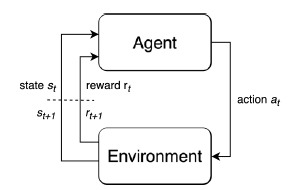
\includegraphics{resources/img/Reinforcement_Learning/RL Control Loop.png}
    \caption{Reinforcement Learning Kontrollfluss \cite{FoundationsDeepRL}}
    \label{fig:rl_control_loop}
\end{figure}
\noindent Abbildung \ref{fig:rl_control_loop} stellt den allgemeinen Markov Entscheidungsprozess (MDP) eines Reinforcement Learning Prozesses dar. Der Agent ist in einer Umgebung (Environment) aktiv. In regelmäßigen Schritten erhält der Agent von der Umgebung einen aktuellen Zustand (State), sowie eine Belohnung (Reward), die entweder Null (d.h. keine Belohnung im aktuellen Schritt), oder ein positiver oder negativer Wert sein kann. Die durch den Agent gelernte Policy bildet den State auf eine Aktion ab. Die Aktion wird in der Umgebung ausgeführt. Danach übergibt die Umgebung den neuen State und die neue Belohnung an den Agenten.\cite{FoundationsDeepRL}

\subsection{Episoden und Trajektorien}
Eine Episode beschreibt die Zeitspanne von der Initialisierung bis zur Terminierung der Umgebung. Eine Trajektorie beschreibt eine Reihe von Tupeln aus State, Aktion und Reward aus den einzelnen Schritten einer Episode. Die Gleichung \ref{eq:trajectory} stellt die mathematische Schreibweise einer Trajektorie dar. Auf Basis gesammelter Trajektorien kann der Agent einen Lernvorgang durchführen und die Policy aktualisieren.\cite{FoundationsDeepRL}
\begin{equation}
    \tau = (s_0,a_0,r_0), (s_1,a_1,r_1), \dots, (s_t,a_t,r_t)
    \label{eq:trajectory}
\end{equation}

\subsection{Policy-basierte \& Value-basierte Algorithmen}
Grundsätzlich wird im Reinforcement Learning zwischen Policy-basierten und Value-basierten Algorithmen unterschieden. Diese werden in den folgenden Abschnitten genauer beschrieben.

\subsubsection{Policy-basierte Algorithmen}
Bei Policy-basierten Algorithmen wählt eine Policy ($\pi$) die nächste Aktion ($a \sim \pi(s)$) aus, die in der Umgebung umgesetzt wird. Diese Policy bzw. ihre Parameter werden direkt durch den Algorithmus gelernt. Es können zwei Arten von Policies verwendet werden. Eine deterministische Policy bildet deterministisch einen Zustand $s$ auf eine Aktion $a$ ab (siehe Gleichung \ref{eq:deterministic_policy}). \cite{FoundationsDeepRL}
\begin{equation}
    \pi(s) = a
    \label{eq:deterministic_policy}
\end{equation}
In der Praxis werden fast ausschließlich stochastische Policies (siehe Gleichung \ref{eq:stochastic_policy}) verwendet.
\begin{equation}
    \pi(a\vert s) = \mathbb{P}_{\pi}\left[ A=a \vert S=s \right]
    \label{eq:stochastic_policy}
\end{equation}
Eine stochastische Policy ordnet für jede Aktion $a$ eine Wahrscheinlichkeit unter Bedingung des Zustands $s$ zu. Aus der entstehenden Verteilung wird dann die Aktion $a$ gesamplet. Policy-basierte Algorithmen lernen die Funktion $\pi$, sodass das Objective maximiert wird.
Policy-basierte Algorithmen können grundsätzlich auf beliebige Aktionstypen angewendet werden, kontinuierliche Aktionsräume sind möglich. Policy-basierte Algorithmen konvergieren garantiert zu einer lokalen, optimalen Policy. Allerdings sind Policy-basierte Algorithmen Proben-ineffizient und haben eine hohe Varianz. \cite{deepRL-2020}

\subsubsection{Value-basierte Algorithmen}
Bei Value-basierten Algorithmen wird eine Funktion zum Schätzen der Wertung eines Zustands bzw. eines Zustand-Aktion Tupels gelernt. Aus der Bewertung wird dann eine Policy generiert. Es gibt zwei grundlegende Value-Funktionen.

\begin{equation}
    V^\pi (s)=\mathbb{E}_{s_0=s, \tau \sim \pi} \left[ \sum_{t=0}^T \gamma^t r_t \right]
    \label{eq:v_function}
\end{equation}
\begin{equation}
    Q^\pi (s,a) = \mathbb{E}_{s_0=s,a_0=a,\tau\sim\pi} \left[ \sum_{t=0}^T \gamma^t r_t\right]
    \label{eq:q_function}
\end{equation}
Die V-Funktion (''Value-Function'', siehe Gleichung \ref{eq:v_function}) schätzt den Wert eines Zustandes anhand der diskontierten kumulativen Belohnung einer in diesem Zustand startenden Trajektorie, unter der Annahme, dass der aktuellen Policy gefolgt wird. 
Die Q-Funktion (''Action-Value-Function'', siehe Gleichung \ref{eq:q_function}) schätzt den Wert eines Zustandes unter Durchführung einer Aktion anhand der diskontierten Rewards einer in diesem Zustand startenden Trajektorie, die zuerst die gewählte Aktion durchführt. 
Bei reinen Value-basierten Algorithmen, wird bevorzugt die Action-Value-Funktion $Q^\pi$ verwendet, da sich diese leichter in eine Policy umwandeln lässt \cite{FoundationsDeepRL}. 
Value-basierte Algorithmen sind Proben-effizienter als Policy-based Algorithmen und haben eine niedrigere Varianz. Allerdings kann eine Konvergenz zu einem lokalen Optimum nicht garantiert werden.

\subsection{REINFORCE}
Der Lernvorgang eines Reinforcement Learning Systems erfolgt über den Policy Gradient.
\begin{equation}
    \vartheta \leftarrow \vartheta + \alpha \nabla_\vartheta J(\pi_\vartheta)
    \label{eq:policy_optimization}
\end{equation}
Gleichung \ref{eq:policy_optimization} zeigt die Optimierung einer Policy. Die optimierte Policy entsteht aus der alten Policy, indem eine Anpassung aus Gradient und Objective Funktion ($J(\pi_\vartheta)$) aufaddiert werden.
\begin{equation}
    \nabla_\vartheta J(\pi_\vartheta) = \mathbb{E}_{\tau\sim\pi_\vartheta} \left[ \sum_{t=0}^T R_t(\tau) \nabla_\vartheta log(\pi_\vartheta(a_t\vert s_t))\right]
    ;\; R_t(\tau) = \sum_{t'=t}^T \gamma^{t'-t} r_{t'}
    \label{eq:gradient_objective_function}
\end{equation}
Dabei werden die Parameter $\pi_\vartheta(a_t\vert s_t)$ der Policy angepasst. Ungünstige Aktionen ($R_t(\tau) < 0$) werden weniger wahrscheinlich. Günstige Aktionen ($R_t(\tau) > 0$) werden wahrscheinlicher. \cite{FoundationsDeepRL}

\subsection{Actor-Critic}
Die Actor-Critic Methode ist eine Methode des Reinforcement Learning. Die Actor-Critic Methode kombiniert die Policy-Gradient und die Value-Function Methoden. Der Actor lernt eine Policy (Policy Gradient Methode) und nutzt für das Lernsignal eine durch den Critic gelernte Value-Function (Value-Function Methode). Durch den Critic wird so eine dichte Bewertungsfunktion erzeugt, auch wenn die echten Rewards aus dem Environment nur selten (d.h. an wenigen Zeitpunkten) vorkommen. 

\subsubsection{Advantage-Actor-Critic (A2C)}
Advantage-Actor-Critic ist eine Variante der Actor-Critic Methode, bei der statt einer Value-Funktion eine Advantage-Funktion verwendet wird.
\begin{equation}
    A^\pi(s_t,a_t) = Q^\pi(s_t,a_t) - V^\pi(s_t)
    \label{eq:advantage_function}
\end{equation}
Die Advantage-Funktion bewertet Zustand-Aktion Tupel im Vergleich zum Durchschnitt des Zustandes. Dadurch wird der erreichbare Reward in Relation zur Ausgangssituation gesetzt. Ein kleiner Reward aus einem schlechten Zustand wird somit ebenso gut gewertet, wie ein großer Reward aus einem guten Ausgangszustand. Überdurchschnittliche Aktionen haben also einen positiven Advantage, während unterdurchschnittliche Aktionen einen negativen Advantage haben.
Durch die Verwendung der Advantage-Funktion ändert sich die Formel für den Gradienten. Die Gradienten Formel für die A2C Methode ist in Gleichung \ref{eq:a2c_gradient} dargestellt.
\begin{equation}
    \nabla_\vartheta J(\pi_\vartheta) = \mathbb{E}_t\left[ A_t^\pi (s_t,a_t) \nabla_\vartheta log(\pi_\vartheta(a_t\vert s_t))\right]
    \label{eq:a2c_gradient}
\end{equation}
Für die Berechnung der Advantage-Funktion werden $V^\pi$ und $Q^\pi$ benötigt. Da es sehr ineffizient ist, sowohl $Q^\pi$, als auch $V^\pi$ zu lernen, lernt der Critic nur $V^\pi$ und schätzt auf dieser Grundlage dann $Q^\pi$. Für die Schätzung kann z.B. Generalized-Advantage-Estimation verwendet werden. \cite{FoundationsDeepRL}

\subsubsection{Generalized-Advantage-Estimation (GAE)}
Generalized-Advantage-Estimation (GAE) ist eine Methode, den Advantage anhand einer gelernten $V^\pi$ Funktion zu schätzen. GAE verwendet einen exponentiell gewichteten Durchschnitt von n-step Forward Return Advantages.
\begin{equation}
    A^\pi_{NSTEP} = \left[ (\sum_{i=0}^n \gamma^i r_{t+i}) + \gamma^{n+1} V^\pi (s_{t+n+1}) \right] - V^\pi(s_t)
    \label{eq:nstep}
\end{equation}
Gleichung \ref{eq:nstep} stellt die Berechnung von n-step Forward Return Advantages dar. Dabei werden $n$ Schritte an tatsächlichen Rewards gewertet. Ab dem $n+1$ Schritt wird mit einer gelernten $V^\pi$ Funktion geschätzt. Die tatsächlichen Rewards sorgen für eine hohe Varianz und haben dafür kein Bias, da sie direkt aus der Umgebung gesamplet werden. Die $V^\pi$ Funktion stellt eine Erwartung über alle möglichen Trajektorien dar und weist damit eine geringe Varianz auf. Da die $V^\pi$ Funktion gelernt wurde, entsteht dabei Bias. Mit kleinen Werten für $n$ haben n-step Forward Return Advantages eine geringe Varianz bei hohem Bias, mit großen Werten für $n$ haben n-step Forward Return Advantages eine hohe Varianz bei geringem Bias (Bias-Variance Trade-Off). Allgemeine Aussagen über die Wahl des $n$ Parameters sind schwierig.\\
Generalized Advantage Estimation hebt die explizite Wahl von $n$ aus, indem n-step Forward Return Advantages für verschiedene $n$ Werte gewichtet. kombiniert werden.
\begin{equation}
    A^\pi_{GAE(\gamma,\lambda)} (s_t,a_t) = \sum_{l=0}^\infty (\gamma\lambda)^l \delta_{t+l} ;\; \delta_t = r_t + \gamma V^\pi (s_{t+1}) - V^\pi(s_t)
    \label{eq:gae}
\end{equation}
Die allgemeine Formel für GAE ist in Gleichung \ref{eq:gae} abgebildet. Die Gewichtung wird durch die Decay-Rate $\gamma \in [0;1]$ und den Discount-Factor $\lambda \in [0;1]$ parametrisiert.
In der Praxis wird statt der unendlichen Summe eine Summe bis zum Ende der verfügbaren Trajektorie verwendet. \cite{gaePaper}


\subsection{Proximal Policy Optimization (PPO)}
Proximal Policy Optimization (PPO) ist ein Reinforcement Learning Algorithmus, der die Actor-Critic Methode umsetzt.

\subsubsection{Performance Collapse}
Ein Problem von Reinforcement Learning Algorithmen ist der Performance Collapse (Leistungseinbruch). Performance Collapse bedeutet, dass die Returns der Umgebung im Lernvorgang plötzlich einbrechen, da z.B. die Policy über ein lokales Optimum heraus optimiert wurde und der Gradient nun zu einem schlechteren lokalen Optimum konvergiert. Die Ursache für das Problem ist der indirekte Ansatz der Policies. Ein RL Algorithmus manipuliert die Parameter der Policy, um diese zu verändern. Kleine Veränderungen in den Parametern können dabei große Veränderungen in der Policy auslösen \cite{FoundationsDeepRL}. Da die Trainingsdaten mit der aktuellen Policy gesammelt werden, kann ein Performance Collapse dazu führen, dass die kollabierte Policy sich nicht mehr erholt. 

% \paragraph{Surrogate Objective}
% Ein Lösungsansatz für das Performance Collapse Problem ist das Einschränken der Größe einzelner Lernschritte. Dieser Ansatz wurde mit dem Trust Region Policy Optimization Algorithmus (TRPO) (\ref{}) eingeführt, auf dem PPO aufbaut. 
% \begin{equation}
%     J(\pi') - J(\pi) = \mathbb{E}_{\tau \sim \pi} \left[ \sum_{t=0}^T \gamma^t A^\pi(s_t,a_t) \frac{\pi'(a_t\vert s_t)}{\pi(a_t\vert s_t)} \right] = J_\pi^{CPI}(\pi')
%     \label{eq:surrogate_objective}
% \end{equation}
% Gleichung \ref{eq:surrogate_objective} zeigt das sogenannte Surrogate Objective $J_\pi^{CPI}$, das von TRPO verwendet wird um die 

\subsubsection{Clipping}
Es gibt zwei theoretische Varianten des PPO Algorithmus. Die erste Variante baut direkt auf dem Trust Region Policy Optimization Algorithmus (TRPO) \cite{trpoPaper} auf und verwendet eine adaptive KL Penalty, um die Schrittgröße einzuschränken. In der Praxis wird jedoch nur die zweite Variante von PPO verwendet, da diese in Tests bessere Ergebnisse erzielt und leichter zu implementieren ist.
Die zweite Variante nutzt ein Clipped Surrogate Objective.
\begin{equation}
    J^{CLIP}(\vartheta) = \mathbb{E}_t\left[ \min(r_t(\vartheta)A_t,clip(r_t(\vartheta),1-\epsilon,1+\epsilon)A_t \right]
    \label{eq:clipped_surrogate_objective}
\end{equation}
Die Gleichung \ref{eq:clipped_surrogate_objective} zeigt das Clipped Surrogate Objective, das vom PPO Algorithmus maximiert wird. Eine Veränderung außerhalb des Bereichs $[1-\epsilon; 1+\epsilon]$ wird dabei geclippt (abgeschnitten) und somit die Schrittgröße eingeschränkt.
\begin{equation}
    J^{CLIP+VF+S}(\vartheta) = \mathbb{E}_t \left[ J_t^{CLIP} - c_1L_t^{VF} + c_2S[\pi_\vartheta(s_t)] \right]
    \label{eq:ppo_objective}
\end{equation}
Die für die Clipped Surrogate Objective Variante des PPO Algorithmus verwendete Loss Funktion wird in Gleichung \ref{eq:ppo_objective} gezeigt. Zusätzlich zum Clipped Surrogate Objective wird der Loss der Value-Funktion und ein Entropie Bonus zur Steigerung der Exploration berechnet. In der Praxis wird das Objective negiert, damit Gradient Descent statt Gradient Ascent durchgeführt werden kann. \cite{PPOPaper}

\paragraph{Algorithmus}

\begin{algorithm}
\begin{lstlisting}[mathescape=true, numbers=left]
for episode=0...MAX do
    for actor=1...N do
        Sample Trajectory for T time steps with $\pi_{\vartheta_{old}}$
        Compute advantage estimates $A_1,\dots,A_T$ with $\pi_{\vartheta_{old}}$
    Collect all states in batch of size N*T
    for epoch=1...K do
        for minibatch of size m in batch do
            Optimize Clipped Surrogate Objective L w.r.t. $\vartheta$
    $\vartheta_{old} = \vartheta$
\end{lstlisting}
\caption{PPO Pseudocode Algorithmus \cite{FoundationsDeepRL}}
\label{alg:ppo}
\end{algorithm}

Algorithmus \ref{alg:ppo} zeigt den Pseudocode des PPO Algorithmus. Für jede Episode wird zuerst pro Actor eine Trajektorie in der Umgebung gesamplet. Dabei werden die Aktionen jeweils durch die aktuelle Policy $\pi_{\vartheta_{old}}$ bestimmt. Für diese Trajektorie werden die zugehörigen Advantages mit GAE berechnet. 
Mit den gesampleten Trajektorien wird die Policy in Epochen trainiert. In jeder Epoche werden Minibatches aus dem gesampleten Batch generiert. Mit den Daten der Minibatches wird das Clipped Surrogate Objective optimiert.

	
	\chapter{Verwandte Arbeiten}

Beschreiben warum andere Quellen nicht ausreichend waren und weshalb der eigene Ansatz jene fehlende Themen ergänzt.

\section{Introduction}
\subsection{ml-Agents} \label{mlAgentsFramework}
Das Unity Machine Learning Agents Toolkit, kurz ml-Agents, ist ein von Unity entwickeltes und unter der Apache License 2.0 lizensiertes open-source Projekt, dass Implementierungen von beliebten Reinforment Learning Algorithmen zur Verfügung stellt.
Das Toolkit wurde am 19. September 2017 vorgestellt und wurde seitdem stetig weiterentwickelt. Die aktuellste Version ist Release 19, welcher am 14. Januar 2022 veröffentlicht wurde. Diese Version bietet neben Implementierungen für die Deep Reinforcement Learning Algorithmen PPO, SAC und MA-POCA auch Implementierungen für die Imitation Learning Algorithmen BC und GAIL.\\

\noindent Neben den Implementierungen der Algorithmen stellt das Toolkit auch eine Python API zur Verfügung. Mit dieser API können eigene Agenten mit den zur Verfügung gestellten Algorithmen trainiert werden. Dabei unterstützt die API sowohl Diskrete als auch Kontinuierliche Aktions- und Beobachtungsräumne. Es unterstützt außerdem das Platzieren von mehreren Agenten in einer Umgebung. Diese können sowohl das selbe Verhalten lernen, um das Training zu beschleunigen, oder verschiedene Verhalten, zum Beispiel zum Trainieren der Charaktere in asymmetrischen Spielen. \\

\noindent Neben der nach der Python API erstellten Umgebung benötigt ml-Agents zum Starten des Trainingsvorgangs noch eine Konfigurations Datei. Diese wird für ml-Agents als eine yaml Datei zur Verfügung gestellt. Diese Datei beinhaltet eine Liste von Verhalten und jeder Agent in der Umgebung muss einem der Verhalten entsprechen. Dies ermöglicht es für verschiedene Verhalten verschiedene Konfigurationen für den Ablauf des Trainings und den Aufbau des Netzwerks anzugeben. 
Die Konfiguration definiert den zu verwendenden Algorithmus, die Anzahl der Schritte, die während des Trainings in der Umgebung ausgeführt werden sollen, und wie oft Checkpoints des Netzes gespeichert werden sollen. Zusätzlich beinhaltet es verschiedene Abschnitte, die Teilaspekte des Trainings beeinflussen. \\
Der Hyperparameter Abschnitt der Datei beschreibt die Parameter des Trainings, wie die Batchgröße, die Buffergröße und die globalen Parameter des ausgewählten Algorithmus, wie zum Beispiel die Lernrate oder das beta und epsilon, bei PPO, oder das tau, bei SAC. \\
Der Network Settings Abschnitt beschreibt die Größe und Anzahl der Schichten in dem Netzwerk. Zusätzlich kann hier angegeben werden, ob die Werte normalisiert werden sollen.\\

\noindent Sowohl die Checkpoints als auch das finale Netzwerk werden als onnx Datei gespeichert, die dann, zum Beispiel mit Unity Barracuda, geladen werden kann, um das Netzwerk zu verwenden.\\
Zum Analysieren und Bewerten des Trainings erhebt ml-Agents während des Trainings verschiedene Daten, wie den durchschnittlichen Reward und die Loss Werte der verschiedenen Netzwerke. Diese werden in einem Tensorboard gespeichert, welches in dem selben Ordner wie die onnx Datei gefunden werden kann. 

\subsection{neroRL}\label{neroRLFramework}

NeroRL ist ein unter der MIT Lizenz lizensiertes Reinforment Learning Framework, dass seinen Fokus auf verschiedene Varianten des Proximal Policy Optimization (PPO) Algorithmus legt. Es basiert auf dem Code von dem ml-Agents Toolkit und verwendet dessen Python API, um mit den Umgebungen zu kommunizieren. \\
NeroRL stellt neben der regulären Variante von PPO auch eine Implementierung mit Rekkurenz zur Verfügung. Zusätzlich kann bei allen Implementierungen der Agent entweder mit geteilten oder mit getrennten Netzwerken und Gradienten für den Aktor und den Kritiker trainiert werden. \\
Diese Implementierungen können verwendet werden, um in der bereits existierenden ObstacleTower Umgebung oder in beliebigen openAIGym Umgebungen zu trainieren. Durch das aufbauen auf dem ml-Agents Toolkit können zusätzlich auch Agenten in Umgebungen trainiert werden, die mit der Python API von ml-Agents erstellt wurden.\\
Allerdings stellt NeroRL noch einige zusätzliche Anforderungen an diese Umgebungen. So dürfen die Observationsräume nur Vektor und Visuelle Beobachtungen enthalten. Außerdem werden nur Diskrete und Multidiskrete Aktionsräume unterstützt. NeroRL kann also nicht verwendet werden, um Agenten in einer Umgebung mit kontinuierlichen Aktionsräumen zu trainieren.
Des weiteren unterstützt neroRL nur genau einen Agenten pro Umgebung. Es ist also nicht möglich das Training zu beschleunigen, indem mehrere Agenten in einer Umgebung das selbe Verhalten lernen. Zum Beschleunigen des Trainings kann bei neroRL stattdessen über ein Attribut in der Konfigurationsdatei angegeben werden, dass mit mehreren Instanzen der Umgebung gleichzeitig trainiert werden soll. So würden bei neroRL zum Beispiel anstelle von einer Umgebung mit zehn Agenten zehn Instanzen der Umgebung mit je einem Agenten ausgeführt.\\

\noindent Zum Starten des Trainingsvorgangs muss dem Framework eine Konfigurationsdatei im yaml Format übergeben werden, welche alle relevanten Informationen für das Training enthält.\\
Der erste Abschnitt enthält Informationen über die Umgebung. Wenn für das Training in Build verwendet werden soll, dann wird der Pfad dazu hier angegeben. Außerdem können in diesem Abschnitt die Reset Parameter angegeben werden.\\
Der zweite Abschnitt enthält die Informationen über das Netzwerk. Dazu gehören neben der Anzahl der Ebenen und deren Größe
auch die Aktivierungs und Kodierungsfunktionien. Der Pfad unter dem das Model gespeichert werden soll und der Abstand der Checkpoints wird ebenfalls in diesem Abschnitt festgelegt.\\
Der dritte Abschnitt beinhaltet Informationen zur Evaluierung eines Modells. Dazu gehört mit wie vielen Instanzen evaluiert werden soll und mit welchen Seeds.\\
Im vierten Abschnitt wird festgelegt wie viele parallele Instanzen der Umgebung zum trainieren verwendet werden sollen und wie viele Schritte jede Instanz pro Update machen soll. Das Produkt dieser beiden Werte ergibt die Batchgröße für das Training.\\
Der letzte Abschnitt enthält die Informationen zum eigentlichen Training. In diesem Abschnitt werden der zu verwendende Algorithmus und die Werte für die Hyperparameter von diesem festgelegt. Die Anzahl an durchzuführenden Updates und die Anzahl an Epochs pro Update werden ebenfalls in diesem Abschnitt festgelegt.\\

\noindent Zum Analysieren und Bewerten erhebt neroRL während des Trainings verschiedene Kenndaten, wie den durchschnittlichen Reward und die Loss Werte der verschiedenen Netzwerke. Diese werden in einem Tensorboard gespeichert, welches standardmäßig in einem summaries Ordner zu finden ist.

	
	\chapter{Fachliches Vorgehen}
\label{Fachliches_Vorgehen}

Keine technischen Details (wie z.B. Implementierung)

\section{Projektorganisation}

Wie sind wir vorgegangen... auf alles bezogen. Wer hat an welchen Kapiteln mitgearbeitet.

\subsection{Creature Animator}
% Carsten
Die Gruppe der Creature Animator hat sich in zwei Untergruppen aufgeteilt. In der ersten Phase hat sich die erste Untegruppe damit beschäftigt, den ML-Agents Walker in eine neue Trainingsumgebung einzubauen und die Skripte dynamischer zu gestalten, damit diese in der zweiten Arbeitsphase verwendet und erweitert werden konnten. Währenddessen versuchte die andere Untergruppe den ML-Agents Walker das Schlagen beizubringen. Die beiden Untergruppen haben sich wöchentlich mittwochs getroffen, um von ihren Fortschritten und Problemen zu berichten. Dabei wurden die Ergebnisse in Protokollen festgehalten, welche in einem GitHub Wiki abgelegt wurden.

In der zweiten Phase, welche nach der Bereitstellung der ersten generierten Kreaturen von der Creature Generator Gruppe begann, veränderten sich die Aufgabenbereiche der beiden Untergruppen. Die \enquote{Schlagen}-Gruppe arbeitete seit dem an einer Erweiterung von Nero-RL, sodass Nero-RL anstelle von ML-Agents zum Trainieren der Kreaturen genutzt werden kann. Die Aufgabe der \enquote{Trainingsumgebung}-Gruppe war es den neuen Kreaturen das Fortbewegen beizubringen und der Creature Generator Gruppe Feedback zu den Kreaturen zu geben. Dabei arbeiteten die Gruppenmitglieder an verschiedenen kleineren Aufgaben. Jan beschäftigte sich mit dem Training und dem Finden und Ausprobieren neuer Rewardfunktionen, Nils arbeitete an der dynamischen Generierung von Arenen und dem Landen von Konfigurationeinstellungen aus Dateien und Carsten testete verschiedene Parameter aus und implementierte das Erstellen von NavMeshes zur Laufzeit. In der zweiten Phase lösten \enquote{On-Demand}-Treffen die regelmäßigen Treffen zwischen den beiden Untergruppen ab, um mehr Zeit zum Arbeiten an den Aufgaben zu haben. Zudem wurden anstelle der Treffen nur noch die wichtigsten Punkte protokolliert. Ansonsten wurden Probleme und Fehler direkt als Issue in den entsprechenden GitHub Repositories hinterlegt.  
\begin{table}[]
	\centering
	\begin{tabular}{l|l}
		\begin{tabular}[c]{@{}l@{}}\enquote{Trainingsumgebung/Movement}-Gruppe\end{tabular} & \enquote{Schlagen/Nero-RL}-Gruppe \\ \hline
		Carsten Kellner                                                       & Jannik Stadtler  \\
		Jan Beier                                                             & Niklas Haldorn   \\
		Nils Dunker                                                                 &                 
		\end{tabular}
		\caption{Die zwei Untergruppen und ihre Mitglieder}
	\end{table}

\DeclarePairedDelimiter\norm{\lVert}{\rVert}

\section{Creature Generation}
\subsection{Parametrische Kreatur}
Als Grundlage für die parametrische Generierung der Kreaturen dient das von Jon Hudson in seiner Thesis \cite{Hudson2013CreatureGU} beschriebene Modell, welches in Abschnitt \ref{} näher beschrieben wird.\\
Die Kreatur besteht aus mehreren Körperteilen, die separat generiert werden und jeweils ihre eigenen Parameter besitzen. Diese Körperteile sind Torso, Beine, Arme, Hals, Füße und Kopf, die jeweils aus einem oder mehreren Knochen bestehen. Alle in diesem Abschnitt erwähnten Zufallsvariablen entstammen einer uniformen Verteilung.

\subsubsection{Knochen Koordinaten}
Um einfache lokale Transformationen zu ermöglichen, definieren wir ein einheitliches Koordinatensystem für alle Knochen. Der Ursprung dessen ist der \textbf{proximale Punkt}, dieser ist der der Körpermitte am nächsten gelegene Punkt und entspricht somit der Stelle, an der der knochen, gegebenenfalls mit einem Offset, an seinem Elternknochen befestigt ist. Der \textbf{distale Punkt} ist der Endpunkt des Knochens, also der am weitesten von der Körpermitte entfernte Punkt. \\ Die \textbf{proximale Achse} verläuft parallel zum Knochen, von der Körpermitte weg, also in Richtung des distalen Punktes. Die \textbf{ventrale Achse} liegt orthogonal zur proximalen Achse und zeigt in Richtung der Vorderseite des Knochens. Diese lässt sich prinzipiell beliebig definieren, in unserem Fall haben wir uns jedoch für Armknochen auf die dem Körper zugewandte Innenseite des Knochens festgelegt, für parallel zum Boden generierte Torsi auf die Unterseite und für alle weiteren Knochen auf die der Blickrichtung des Skeletts zugewandten Seite. Die \textbf{laterale Achse} liegt senkrecht auf den beiden zuvor definierten Achsen.

\subsubsection{Generierung}
Unsere Methode setzt voraus, dass zunächst gewisse Vorgaben zur generellen Struktur der Kreatur gemacht werden. In unserem konkreten Fall bedeutet dies, dass wir uns zunächst auf Zwei- und Vierbeiner beschränken. Der Zweibeiner orientiert sich an der menschlichen Anatomie und besitzt deshalb in jedem Bein jeweils zwei Knochen und einen einzelnen Fußknochen sowie zwei Arme. Die Beine eines Vierbeiners besitzen, angelehnt an die Skelette echter vierbeiniger Säugetiere, jeweils vier Knochen. Arme werden hier nicht generiert. Um Kreaturen zu erzeugen, die nicht einer dieser Strukturen entsprechen, wie beispielsweise Spinnentiere oder Echsen, müsste man weitere Skelette definieren.\\
\\
Zuerst  wird der \textbf{Torso} Generiert. Im Falle des Zweibeiners ist dieser nach oben gerichten, beim Vierbeiner parallel zum Boden. Als Parameter werden jeweils Minima und Maxima für die Länge und den Umfang des Torsos übergeben. Daraus wird zunächst ein zufälliger Wert für die Länge bestimmt. Da wir uns vorerst für einen Torso bestehend aus drei Knochen entschieden haben, wird diese Länge zufällig auf drei kleinere Längen aufgeteilt. Jeder dieser Knochen erhält dann einen zufälligen Umfang. Das unterste Torsosegment dient als Elternknochen der Kreatur, die anderen beiden Knochen werden dann nacheinander am distalen Punkt des vorangegangenen Knochens befestigt.\\
Anschließend werden die \textbf{Beine} paarweise generiert, wodurch nur symmetrische Kreaturen erstellt werden können. Auch hier wird zunächst die Länge zufällig bestimmt und dann auf zwei beziehungsweise vier Knochen aufgetelt. Auch Die Umfänge werden zufällig bestimmt, jedoch zusätzlich sortiert, sodass das das dickste Segment der Körpermitte am nächsten gelegen ist. In beiden Fällen werden die Beine gerade nach unten gereriert. Bei einem Zweibeiner wird am distalen Punkt des unteren Beinknochen in Richtung dessen ventraler Achse ein Fußknochen mit parametrisch zufällig bestimmter Größe erzeugt. Befestigt werden die Beine durch einen zusätzlichen Hüftknochen, der parallel zum Torso am proximalen Punkt des ersten Torsoknochens ansetzt und dessen proximale Achse entgegen derer seines Elternknochens gerichtet ist, also den Torso etwas verlängert. Es wird jeweils ein Bein links und rechts vom Mittelpunkt des Hüftknochens angebracht. Der Abstand entlang der lateralen Achse ergibt sich aus dem Umfang des Knochens. Im Falle des Vierbeiners wird analog dazu ein weiteres Beinpaar am distalen Punkt des letzten Torsoknochens generiert. Anschließend werden Torso und Beine so rotiert, dass sich alle Enden der Beine auf der selben Höhe befinden und die Beine noch immer gerade nach unten Zeigen.\\
Die \textbf{Arme} des Zweibeiners werden analog zu den Beinen mit Hilfe eines Schultersegmentes am distalen Punkt des obersten Torsoknochens erzeugt.\\
Der \textbf{Hals} wird als Verlängerung des Torsos generiert. Dabei wird sowohl die Länge und Dicke zufällig bestimmt als auch die Anzahl der Knochen. Beim Zweibeiner wird er am distalen Punkt des Schulterknochens befestigt und alle Knochen zeigen parallel zum Torso gerade nach oben. Beim Vierbeiner erfolgt das Befestigen am distalen Punkt des vorderen Hüftknochens. Dabei ist die Rotation des ersten Knochens ein zufälliger Wert zwischen der der proximalen und der der negativen ventralen Achse des Elternknochens. Jedes weitere Halssegment erhält eine zufällige Rotation um $\pm 20\degree$.\\
Der \textbf{Kopf} ist ein einzelner Knochen mit zufälliger Länge und Umfang, der als Verlängerung des letzten Halsknochens betrachtet werden kann.\\
\\
Die glaubwürdigkeit und Variation der Kreaturen ist dadurch also auch stark von den gewählten Parametern Abhängig. Diese werden von Hand gesetzt, wobei größere Wertebereiche auch für größere Unterschiede zwischen den Kreaturen sorgen, aber gleichzeitig die Kontrolle über das Ergebnis einschränken. Die Beschränkungen der Bewegungsradii der Gelenke werden momentan händisch mit erfahrungsgemäß guten Werten gesetzt. Ziel ist es allerdings auch diese in Zukunft soweit möglich prozedural mit Hilfe von Parametern zu erzeugen, um verschiedene Bewegungsmuster zu ermöglichen.




\subsection{L-System Creature}
% Vom L-System zu den Knochen (Strecken) -> Rotation um die Achsen mittels Euler->Quarternion
\subsubsection{Generierung der Skelettstruktur}

%Nach Subsubsection "Generierung der Skelettstruktur"
\subsubsection*{Skelett aus L-System generieren}
Ausgehend von einer Liste von Tupeln, die jeweils Start und Endpunkte einer von der Turtle gezeichneten Strecke enthalten wird das Skelett mit Unity Klassen generiert. Zunächst wird die Liste in eine Baumstruktur überführt. Dabei entspricht ein Knoten im Baum einem Knochen im Skelett. Zwei Knoten stehen in einer Eltern-Kind-Beziehung im Baum, wenn die zugehörigen Strecken sich schneiden. Dabei wird gefordert, dass der Endpunkt der zum Elternknoten gehörigen Strecke dem Startpunkt der zum Kindknoten gehörigen Strecke gleicht. Da angenommen wird, dass es zu jedem Startpunkt eines Tupels in der Liste ein weiteres Tupel gibt, dessen Endpunkt dem Startpunkt gleicht lässt sich der Baum so definieren. Der Baum wird traversiert und zu jedem Knoten wird ein GameObject erstellt.  Dieses wird mit einem Rigidbody, einem CapsuleCollider und einem primitiven Mesh versehen. Die Knochen werden in Kategorien, wie zum Beispiel Arm, Bein oder Kopf eingeteilt. Zwei Knochen werden mit einem Joint verbunden, wenn sie im Baum in einer Eltern-Kind-Beziehung stehen. Für die erlaubten Rotationen der Joints wurden Standardwerte je nach Kategorie festgelegt. Abbildung \ref{skeletonlsystemex} zeigt ein über ein L-System generiertes Skelett.

\begin{figure}[h]
\begin{center}
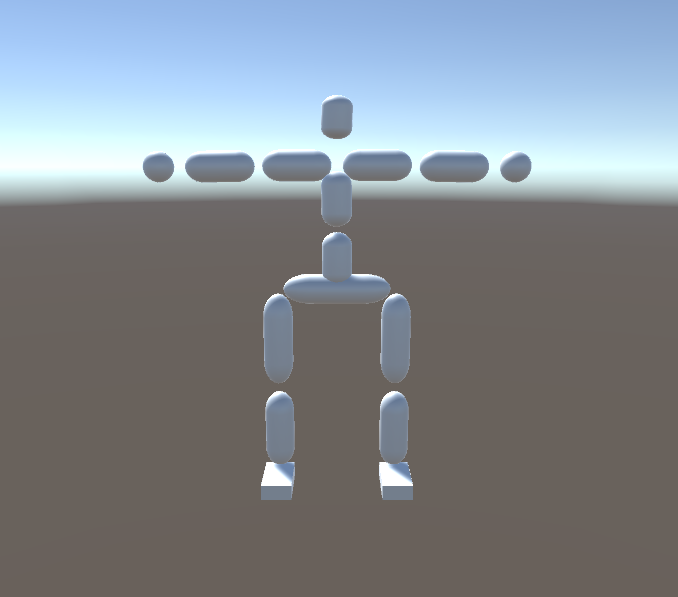
\includegraphics[width = 0.5\textwidth]{resources/img/skeletonlsystemex.png}
\end{center}
\caption{Mittels L-System generiertes Skelett}
\label{skeletonlsystemex}
\end{figure}


\subsection{Mesh-Generierung}
\subsubsection{Metaball}
Zur Generierung der Geometrie der Kreatur verwenden wir, angelehnt an den Ansatz von Madis Janno \cite{Janno20182dCG} (siehe Abschnitt \ref{sec:metaball}), eine modifizierte Form von Metaballs. Dabei werden genau so viele Bälle entlang eines Generierten Segments platziert wie benötigt werden um zu garantierten, dass dadurch in jedem Fall ein zusammenhängendes Mesh entsteht. Tatsächlich ist jedoch der Einfluss nahegelegener Kugeln aufeinander so groß, dass dadurch nicht nur die minimale Berührung der einzelnen Kugeln entsteht, sondern diese glatt ineinander übergehen. Wie auch bei Janno lässt sich unsere Methode mit beliebigen Metaball-Funktionen durchführen. Aufgrund der guten Ergebnisse haben wir uns jedoch vorerst auf die gleiche, zuerst von Ken Perlin beschriebene, Falloff-Funktion festgelegt.
\[f_i(\vec{x}) = exp(B_i - \frac{B_ir_i^2(\vec(x))}{R_i^2})\]
Für Metaball $i$ ist $R_i$ dessen Radius, $B_i$ ein Parameter zur Einstellung der "Blobbiness", welcher beeinflusst wie sehr sich Metaballs miteinander verbinden. Wir verwenden den Wert $B_i = 0.5$. $r_i(vec{x})$ ist der Abstand des Punktes $\vec{x}$ zum Zentrum $c_i$ von Metaball $i$, also: \[r_i(\vec{x})=||\vec{x}-\vec{c_i}||=\sqrt{(x_x-c_{ix})^2+(x_y-c_{iy})^2+(x_z-c_{iz})^2}\]

Die generierten Kreaturen bestehen aus mehreren Segmenten (Knochen) mit jeweils einem Start- und Endpunkt sowie einer Dicke, die als Radius der darauf platzierten Metaballs verwendet werden kann. Entlang dieser Segmente soll dann das Mesh erzeugt werden. Die von Janno beschriebene Methode berechnet dafür, abhängig von der gewählten Falloff-Funktion, die minimale Anzahl an Metabällen für ein Segment und platziert diese gleichmäßig entlang dessen. Das Problem, welches sich daraus bei unseren Experimenten ergeben hat, liegt darin, dass mit höherer Komplexität der Kreaturen und einer damit einhergehenden steigenden Anzahl an Segmenten, der Einfluss von benachbarten Segmenten nicht gut kontrollieren lässt und diese teilweise ineinander verschmelzen. \\

Unser Ansatz um dieses Problem zu umgehen ist es, die Anzahl der einzelnen Metabälle drastisch zu reduzieren. Anstatt einer beliebig großen Zahl an Bällen entlang jedes Segments, erzeugen wir jeweils nur einen einzigen Körper. Dazu ersetzen wir die Bälle durch Kapseln, also Zylinder mit jeweils durch eine Halbkugel abgerundeten Enden, weshalb wir diese auch als "Metakaspeln" bezeichnen. Möglich macht uns dies eine Modifikation der Falloff-Funktion, beziehungsweise der darin verwendeten Distanz. Wir berechnen hierbei nicht den Abstand zum Zentrum einer Kugel, sondern zu der Verbindungslinie zwischen Start- und Endpunkt. \\

\begin{figure}[ht]
\centering
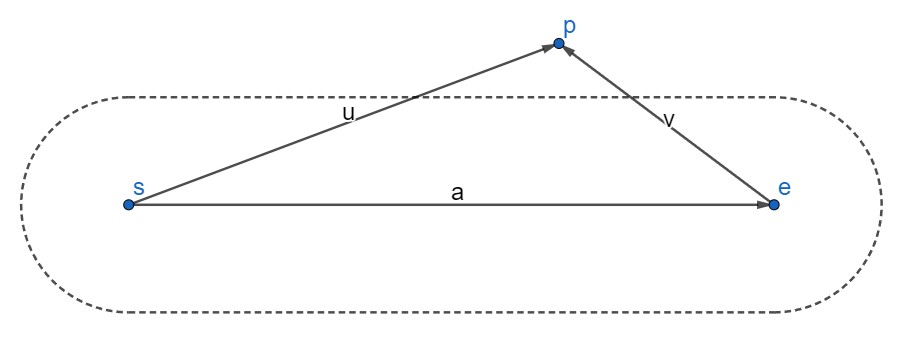
\includegraphics[width=0.7\textwidth]{resources/img/metacapsule.png}
\caption{Beispiel Metakapsel; Die gestrichelte Linie enthält alle Punkte mit $r=R$}
\label{metacapsule}
\end{figure}

Um diese Form zu erzeugen muss lediglich die Funktion $r(\vec{x})$ zur Berechnung des Abstandes angepasst werden.
Sei $s$ der Startpunkt, $e$ der Endpunkt, $a$ der Vektor $e-s$, $p$ ein Punkt, dessen Abstand berechnet werden soll, $u=p-s$ und $v=p-e$ (Siehe Abbildung \ref{metacapsule}). Die Distanz lässt sich dann folgendermaßen bestimmen:
\[
    r(\vec{x})= 
\begin{cases}
    ||p-s||,& \text{falls } a\cdot u < 0\\
    ||p-e||,& \text{falls } a\cdot v > 0\\
    \norm*{\frac{a\times u}{\norm{a}}},& \text{sonst}
\end{cases}
\]

Es werden drei Fälle unterschieden. Liegt der Punkt $p$ im Falle von Abbildung \ref{metacapsule} links von $s$, beziehungsweise rechts von $e$, ist Die Distanz von $p$ zum Segment einfach der euklidische Abstand zum jeweiligen Punkt. Ob dies der Fall ist, lässt sich mit Hilfe der Skalarprodukte $a\cdot u$ beziehungsweise $a\cdot v$ überprüfen. Ansonsten berechnet man die Distanz von Punkt p zur Geraden, die durch $s$ und $e$ verläuft.\\

Da dies nur eine Erweiterung der Metaball-Funktion ist, lassen sich diese Kapseln weiterhin mit anderen Metabällen kombinieren. So können auch Körperteile erstellt werden, die nicht aus solchen Segmenten bestehen, oder Details aus kleineren Metabällen entland der Segmente platziert werden. Grundsätzlich lassen sich auf diese Weise beliebig geformte Objekte, die mit einer solchen Funktion definiert werden, einbinden.
Da die Kapsel nur zylindrisch geformte Segmente darstellen lässt, die in alle Richtungen den gleichen Radius besitzen, haben wir eine weitere Modifikation vorgenommen, die es erlaubt die Metakapsel entlang der ventralen oder lateralen Achse zu strecken beziehungsweise zu stauchen. Dadurch ist es uns möglich Körperteile mit unterschiedlichen Abmessungen entlang der verschiedenen Achsen darzustellen und dennoch unnatürlich wirkende Formen wie beispielsweise einen Quader zu vermeiden.
Dazu bestimmen wir bei der Berechnung von $r(\vec{x})$ zunächst den Vektor, der die kürzeste Verbindung von $\vec{x}$ und dem Segment darstellt, anstatt direkt dessen Länge auszuwerten. Diesen Vektor skalieren wir anschließend entlang der gewünschten Achse. Die Länge des skalierten Vektors ist dann die neue Distanz.


\subsubsection{Marching Cubes}
TODO: wollen wir hier noch etwas genauer drauf eingehen, oder reicht der Teil von Jona???

\subsubsection{Mesh Indexing}
Zur weitere Verarbeitung des Meshes beim automatischen Rigging, ist es wichtig, dass das Mesh korrekt indiziert ist, sodass keine doppelten Vertices existieren. Außerdem können so die ausgehenden Kanten der Vertices bestimmt werden, welche ebenfalls später für das automatische Rigging benötigt werden. Während dem Marching Cubes Algorithmus werden die entstehende Dreiecke in eine gesonderte Datenstruktur hinzugefügt, welche für jeden Vertex prüft, ob dieser bereits im Vertex-Buffer existiert. Falls ja, wird kein neuer Vertex eingefügt, sondern das Dreieck referenziert den Vertex über den Index-Buffer. Neue Vertices werden dem Vertex-Buffer hinzugefügt und das entsprechende Dreieck referenziert den neuen Vertex. Die Anzahl der Vertices wird dadurch außerdem signifikant verringert, was Performance-Vorteile beim Rendering und bei der Weiterverarbeitung des Meshes ermöglicht.

\subsubsection{Delaunay Triangulation}
In der Entwicklung des automatischen Riggings des Modells wurde festgestellt, dass die Triangulierung, die durch Marching Cubes entsteht nicht geeignet ist, um mit der Bone-Heat Methode die Vertex-Gewichte zu berechnen. Für die Lösung des Matrix-Systems der Bone-Heat Methode ist es wichtig, dass die Triangulierung die Delaunay-Bedingung erfüllt.

TODO: Delaunay Edge-flipping Algorthmus erklären

\subsection{Automatisches Rigging}
Um die Bone-Struktur des generierten Skelettes mit dem Mesh zu verknüpfen, muss bei der 3D-Modellierung der Prozess des Riggings durchlaufen werden. Dieser beschreibt wie sich jeder einzelne Vertex des Meshes mit den Bones in der Szene bewegt. Jeder Vertex kann an beliebig vielen Bones angehängt werden. Durch eine Gewichtung wird bestimmt wie sehr ein Vertex durch der Transformation eines Bones mitbewegt wird.
Da sowohl das Skelett, als auch das gesamte Mesh prozedural generiert werden, kann das Rigging nicht wie üblich in einem Modellierungs-Tool wie Blender~\cite{blender} manuell durchgeführt werden, sondern muss zur Laufzeit des Spiels während der Generierung der Kreaturen geschehen.

Für ein erfolgreiches Rigging ist es wichtig, dass das Skelett bereits sinnvoll in dem Mesh eingebettet ist. Da hier das Mesh aus Metaballs generiert wird, welche um die Bones plaziert sind, können wir hier davon ausgehen, dass das Mesh das Skelett bereits \emph{sinnvoll} umhüllt.

\begin{figure}[h!]
	\centering
	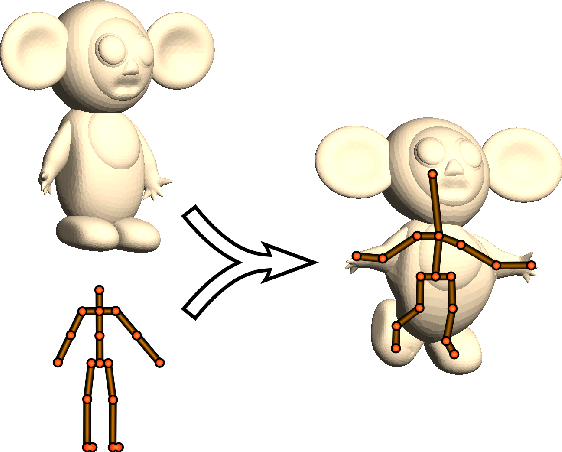
\includegraphics[width=0.6\linewidth]{resources/img/skeleton_embedding.png}
	\caption{Beispiel für ein korrekt eingebettetes Skelett in einem Mesh~\cite{bone_heat_paper}.}
	\label{fig:skeleton_embedding}
\end{figure}

Während der Entwickelung wurde zunächst eine triviale Methode als Zwischenlösung verwendet. Dabei wurden alle Vertices nur an den Bone mit der geringsten Distanz angehängt. Diese Methode ist jedoch visuell unbrauchbar, da bei Bewegung des Skeletts an den Gelenken zwischen den Bones Löcher und verschiedene andere Artefakte entstehen. Es wird also eine Lösung benötigt, die es ermöglicht Vertices an mehrere Bones anzuhängen und die Gewichte so bestimmt, dass das Mesh an den Übergängen zwischen den Bones möglichst natürlich deformiert wird.

\subsubsection{Bone-Heat Methode}
Ein bereits bekannter Algorithmus zur automatisch Gewichtsberechnung und Verknüpfung des Meshes ist die Bone-Heat Methode~\cite{bone_heat_paper}. Dieser berücksichtig mehrere zusätzliche Eigenschaften für die Gewichte. Zuerst sollen die Gewichte unabhängig von der Auflösung des Meshes sein. Außerdem müssen die Gewichte sich sanft über den Verlauf der Oberfläche verändern. Die Breite des Übergangs zwischen zwei Bones sollte ungefähr proportional zu der Distanz des Gelenks zur Oberfläche des Meshes sein.
Ein Algorithmus, welcher die Gewichte alleine aus der Distanz der Bones zu den Vertices berechnet, kann oft schlechte Ergebnisse liefern, da er die Geometrie des Modells ignoriert. Zum Beispiel können Teile des Torsos mit einem Arm verbunden werden. Die Bone-Heat Methode behandelt stattdessen das innere Volumen des Modells als einen wärmeleitenden Körper. Es werden für jeden Vertex die Gleichgewichts-Temperatur berechnet und diese als Gewichte für die Bones verwendet. Wie in Abbildung~\ref{fig:bone_heat_equilibrium} zu sehen ist, wird ein Bone auf 1° gesetzt und der andere auf 0°. Bei Deformation der beiden Bones mit den Gewichten aus dem Temperatur-Gleichgewichts entsteht an dem Gelenk eine natürlich aussehende Verformung der Oberfläche.

\begin{figure}[h!]
	\centering
	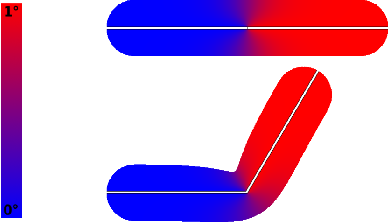
\includegraphics[width=0.7\linewidth]{resources/img/bone_heat_equilibrium.png}
	\caption{Temperatur-Gleichgewicht für zwei Bones~\cite{bone_heat_paper}.}
	\label{fig:bone_heat_equilibrium}
\end{figure}

Das Temperatur-Gleichgewicht des Volumens zu berechnen wäre sehr aufwändig und langsam, deswegen wird das Gleichgewicht nur über die Oberfläche des Meshes berechnet. Die Gewichte für Bone $i$ werden berechnet durch:

\begin{equation}
    \label{eq:bone_heat}
    \begin{aligned}
        &\frac{\partial\mathbf{w}^i}{\partial t} = \Delta\mathbf{w}^i+\mathbf{H}\left(\mathbf{p}^i-\mathbf{w}^i\right)=0 \\
        \iff &-\Delta\mathbf{w}^i+\mathbf{H}\mathbf{w}^i=\mathbf{H}\mathbf{p}^i \\
        \iff &\left(-\Delta+\mathbf{H}\right)\mathbf{w}^i=\mathbf{H}\mathbf{p}^i
    \end{aligned}
\end{equation}

Dabei ist $\Delta$ der diskrete Laplace-Beltrami Operator auf der Oberfläche des Meshes, welcher mit der Kotangens-Methode approximiert wird~\cite{laplace_beltrami_paper}. $\mathbf{p}^i$ ist ein Vektor mit $p^i_j=1$ wenn der nächste Bone zum Vertex $j$ der Bone $i$ ist. Sonst ist $p^i_j=0$. $\mathbf{H}$ ist eine Diagonalmatrix wobei $H_{jj}$ die Hitze des nächsten Bones von Vertex $j$ ist. Sei $d(j)$ die Distanz zum nächsten Bone von Vertex $j$, dann wird $H_{jj}=c/d(j)^2$ gesetzt. Allerdings nur wenn das Geradensegment von dem Vertex zu dem Bone vollständig in dem Volumen des Modells enthalten ist. Wenn der Bone von dem Vertex aus also nicht sichtbar ist, wird $H_{jj}=0$ gesetzt. Dies verhindert, dass beispielsweise Vertices am Arm and den Torso angehängt werden. Wenn mehrere Bones nahezu die gleiche Distanz zu dem Vertex haben und sichtbar sind, werden ihre Anteile an der Temperaturverteilung gleich berücksichtigt. $p_j$ wird dann $1/k$ und $H_{jj} = kc/d(j)^2$

Der benötigte Sichtbarkeits-Test wird durch ein Signed-Distance-Field (SDF) realisiert, welches wir vorab mit einem Geometry-Shader generieren. Damit werden effiziente Raycast-Operationen in dem Mesh möglich. (TODO: passendes Zitat finden)
Der Parameter $c$ wird in dem Paper~\cite{bone_heat_paper} auf $1$ gesetzt, um natürlichere Ergebnisse zu erreichen. Für $c\approx0.22$ würde der Algorithmus Gewichte berechnen die ähnlicher zu dem Temperatur-Gleichgewicht über dem tatsächlichen Volumen des Meshes sind.

\subsubsection{Lösen des Laplace-Beltrami Systems}
Für die effiziente Lösung des Matrix-Systems in Formel \ref{eq:bone_heat} ist es wichtig die Eigenschaften des diskreten Laplace-Beltrami Operators $\Delta$ näher zu betrachten. Der Operator wird durch die Kotangens-Methode approximiert, indem von jedem Vertex $x_i$ für jede ausgehende Kante ein Gewicht $v(x_i,x_j)$ aus den gegenüberliegenden Winkel $\alpha_{ij}$ und $\alpha_{ji}$ berechnet wird (siehe Abbildung~\ref{fig:cotangent_approx}).

\begin{figure}[h!]
	\centering
	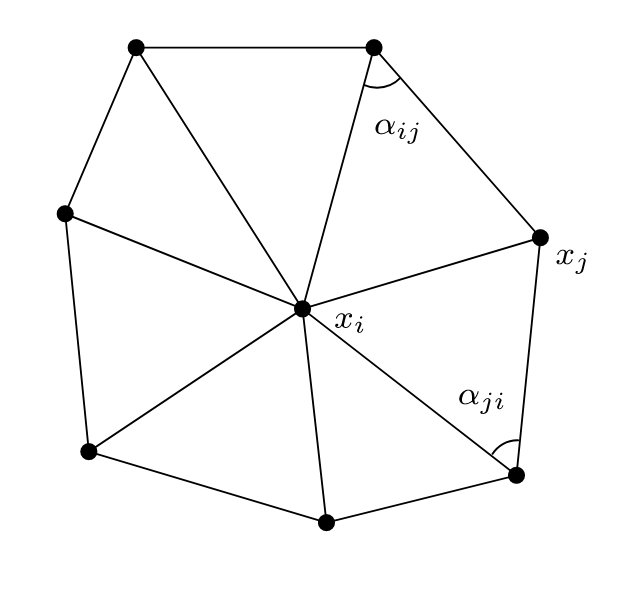
\includegraphics[width=0.4\linewidth]{resources/img/cotangent_approx.png}
	\caption{Berechnung der $\alpha$-Winkel für eine innere Kante~\cite{laplace_beltrami_paper}.}
	\label{fig:cotangent_approx}
\end{figure}

\begin{equation}
    \label{eq:cotangent_weight}
    v(x_i,x_j) = 
        \begin{cases}
            \cot{\alpha_{ij}}+\cot{\alpha_{ji}}\ & \text{for interior edges} \\
            \cot{\alpha_{ij}} & \text{for boundary edges}
        \end{cases}
\end{equation}

Aus den Kotangens-Gewichten aus Gleichung~\ref{eq:cotangent_weight} kann nun in Formel~\ref{eq:laplace_beltrami} der Laplace-Beltrami Operator in seiner Matrix-Form berechnet werden \cite{spd_solver_paper,laplace_beltrami_paper}. Dabei bescheibt $N(x_i)$ die Menge der benachbarten Vertices von $x_i$. Da für das Lösen der Gleichung~\ref{eq:bone_heat} lediglich die Matrix $(-\Delta+\textbf{H})$ benötigt wird, kann diese in der Implementierung direkt als eine Matrix erstellt werden. Die Normalisierungsfaktoren aus~\cite{spd_solver_paper} wurden hier weggelassen, da sie für diese Anwendung sowieso wegfallen.

\begin{equation}
    \label{eq:laplace_beltrami}
    \Delta_{ij}=
    \begin{cases}
        0 & i \neq j, x_j \notin N(x_i) \\
        v(x_i,x_j) & i \neq j, x_j \in N(x_i) \\
        -\sum_{x_j\in N(v_i)} v(x_i,x_j) & i = j\\
    \end{cases}
\end{equation}

Da die Matrix $\textbf{H}$ eine Diagonalmatrix ist und der Operator $\Delta$ eines Vertex durch seine direkten Nachbarn lokal definiert ist, ist die zu lösende Matrix extrem dünn besetzt. Durch die Euler-Charakteristik für Dreiecks-Netze ergeben sich nur ungefähr $7$ Einträge in der Matrix pro Reihe~\cite{spd_solver_paper}. Ein solches System lässt sich, wie in~\cite{spd_solver_paper} gezeigt, sehr effizient lösen, wenn es sich um eine SPD-Matrix (symetrisch positiv definit) handelt. Die Matrix ist durch die Konstruktion symetrisch. 

TODO: Delaunay Bedingung erklären und Verbindung zu Definitheit erklären

TODO: Berechnung und Normalisierung der finale Vertex-Gewichte


\section{Creature Animation}

\subsection{Trainingsumgebung}
% Carsten
Als Grundlage für die eigene Trainingsumgebung diente die Trainingsumgebung des ML-Agent Walkers. Bei genauerer Betrachtung der Trainingsumgebung des ML-Agent Walkers stellte sich sehr schnell raus, dass diese für unsere Anforderungen zu statisch war, da es zum Beispiel nicht möglich war, die verwendete Kreatur einfach gegen eine andere Kreatur auszutauschen. Zudem mussten neue Arenen aufwendig per Hand erstellt werden und die Kreaturen konnten nur auf einer flachen Ebene trainiert werden. Daher wurde eine eigene dynamischere Trainingsumgebung erstellt, die vor allem die zuvor genannten Punkte umsetzt. Sowohl die Anzahl der Arenen als auch die Kreatur können in der neuen Trainingsumgebung einfach eingestellt werden. Somit können die Arenen vollständig zur Laufzeit generiert werden. Zudem besteht die Möglichkeit neben flachen Terrain auch unebenes Terrain zu verwenden.

Zunächst wurde der ML-Agents Walker zum Testen der neuen Trainingsumgebung verwendet, damit die Kreatur als Fehlerquelle ausgeschlossen werden konnte. Nachdem die Tests mit dem ML-Agents Walker erfolgreich waren, wurde der ML-Agents Walker durch eine neue Kreatur ersetzt, welche mit Hilfe des L-Systems zuvor generiert wurde. Die neue Kreatur wurde ausgiebig in der neuen Trainingsumgebung getestet und mit dem ML-Agents Walker verglichen. Durch das dadurch gewonnene Feedback konnte die Creature Generator Gruppe Anpassungen und Verbesserungen an der Kreatur vornehmen.

Trotz den vielen Änderungen an der Kreatur war es nicht möglich, die Kreatur aus dem L-System zum Laufen zu bringen. Aus diesem Grund ersetzte eine andere Methode, welche von Jona und Markus umgesetzt wurde, das L-System. Mit der neuen Methode wurde auch der Creature-Generator direkt in die Trainingsumgebung eingebunden. Dies ermöglichte es, schnell verschiedene Kreaturen zu testen. Die Bugreports und Featurerequests zum Generator werden direkt als Issue in das entsprechende GitHub Repository geschrieben und werden gegebenenfalls im Jour Fixe oder über Discord besprochen.



\section{Terraingeneration}
	
	\chapter{Technische Umsetzung}
Bei der Erläuterung der Wahl der Hierarchie für Knochen nur deskriptiv darauf eingehen; keine Details oder Begründung erforderlich. \textbf{Dies übernimmt die Creature-Generator Gruppe.}
Eingehen auf Status Quo.
\section{Creature Animation}
% !TeX spellcheck = de_DE

\subsection{Trainingsumgebung}
Im Folgenden soll der Aufbau der Trainingsumgebung beschrieben werden, welche es erlaubt verschiedenste Kreaturen ohne große Anpassungen zu trainieren. Im Laufe der Projektgruppe wurden drei unterschiedliche Versionen der Trainingsumgebung genutzt. 

\subsubsection{Vorherige Versionen}
Die erste Version ist eine leicht abgeänderte Form der ML-Agents-Beispielumgebung für den Walker. Dabei handelt es sich um eine Unity-Szene mit einer fest vorgebenden Anzahl an Arenen und Kreaturen, welche trainiert werden können.

Da sich hier schnell Limitationen in Bezug auf die Anpassbarkeit herausstellten wurde die Umgebung geändert, so dass die Anzahl der Arenen dynamisch generiert werden und Kreaturen als Prefab und per Seed über den \texttt{CreatureGenerator} platziert werden können. 

Die  \texttt{DynamicEnviormentGenerator}-Umgebung ist dabei aus den folgenden Klassen aufgebaut:

\begin{itemize}
	\item \texttt{DynamicEnviormentGenerator}
	\begin{itemize}
		\item \texttt{TerrainGenerator} %Todo change when replaced by package
		\item Verschiedenen Konfigurationsdateien
		\item \texttt{DebugScript}
	\end{itemize}
	\item großteils alle modifizierten ML-Agents Skripten
\end{itemize} 

Da die Umgebung weiterhin als zusätzliche Szene in dem Projekt existiert\footnote{Es sei dabei angemerkt, dass die Szene nicht aktiv getestet wird und deswegen nicht garantiert werden kann, dass mit weiteren Änderungen die Funktionalität bestehen bleibt.} und die aktuelle Version der Trainingsumgebung auf dem \texttt{DynamicEnviormentGenerator} aufbaut, wird im Folgenden auf den Aufbaue des \texttt{DynamicEnviormentGenerator} sowie dessen Hilfsklassen eingegangen. Die Hilfsklassen sind der \texttt{TerrainGenerator}, \texttt{GenericConfig} und dessen Implementierungen sowie das \texttt{DebugScript}. Erstere ist verantwortlich für die Generierung des Terrains, die Config-Dateien laden dynamisch die Einstellungen aus einer Datei und das letzte Skript beinhaltet hilfreiche Debug-Einstellungen. Die grundsätzliche Idee der Trainingsumgebung stammt von dem ML-Agents-Walker. Da an diesem keine Versuche mit Unterschiedlichen Umgebungen und Kreaturen durchgeführt wurden, ist der Aufbau des Projekts nicht dynamisch genug. 

\paragraph{Dynamic Enviorment Generator}
\begin{figure}
	\centering
	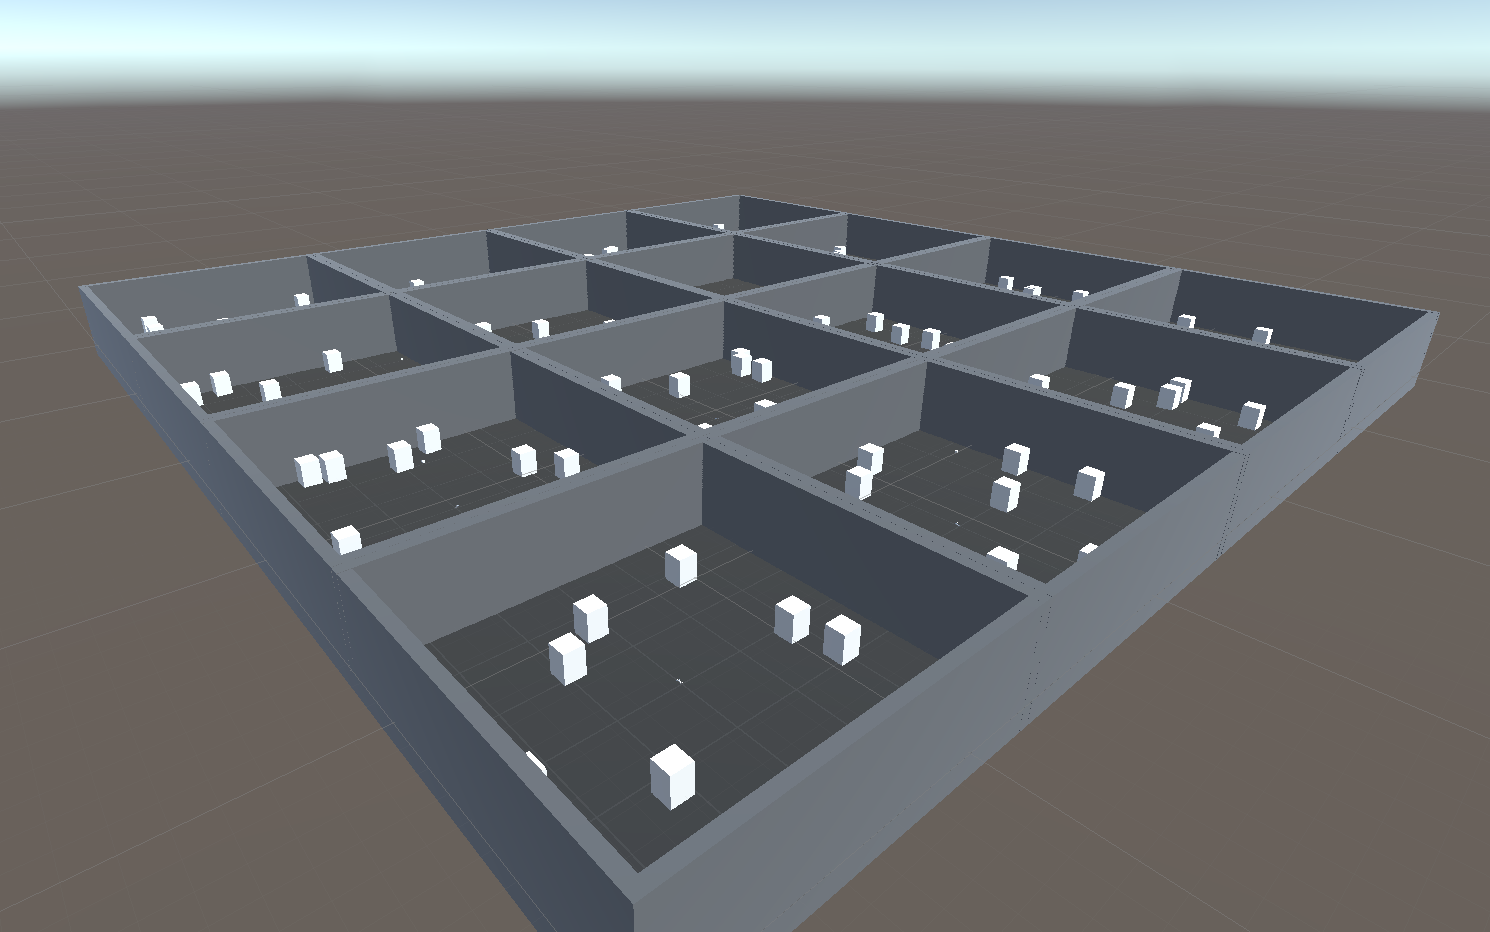
\includegraphics[width=0.7\linewidth]{resources/img/DEGArenen}
	\caption[Beispiel der generierten Trainingsumgebung]{Ein Beispiel der generierten Trainingsumgebung mit mehreren Arenen.}
	\label{bspArena}
\end{figure}
Zur dynamischen Umsetzung der Trainingsarena werden alle Objekte zur Laufzeit erstellt. Die Generierung der Arena läuft dann wie folgt ab:
\begin{enumerate}
	\item Erstellen von $n$ Arenen, wobei $n$ eine zu setzende Variable ist. 
	\item Füge ein Ziel für die Kreatur in die Arena ein
	\item Generiere die Kreatur
\end{enumerate} 
Die einzelnen (Teil)-Arenen, abgebildet in der Grafik \ref{bspArena}, bestehen aus einem Container-Objekt unter dem ein Terrain und vier Wall-Prefabs angeordnet sind. Diese Prefabs und weitere Elemente wie Texturen werden dynamisch aus einem Ressourcen-Ordner geladen, damit möglichst wenige zusätzliche Konfigurationen den Editor verkomplizieren. Das Terrain wird mit leeren Terraindaten vorinitialisiert und später befüllt. Hierbei kann die Position des Container-Objects in der Szenen wie folgt berechnet werden:
\begin{align}
	\begin{pmatrix}
	\lceil \frac{\text{Anzahl der Arenen}}{\sqrt{\text{Anzahl der Arenen}}} \rceil \\
	0 \\
	\text{Anzahl der Arenen} \mod \sqrt{\text{Anzahl der Arenen}} \\
	\end{pmatrix}
	 = 	\begin{pmatrix}
	 x  \\
	 y \\
	 z  \\
	 \end{pmatrix}
\end{align}
Alle anderen Objektpositionen müssen danach neu im lokalen Koordinatensystem gesetzt werden. Da die Unity-Standard-Texturen sehr hell sind sind, werden die Texturen bei der Initialisierung mit ML-Agents-Texturen, welche dunkler sind, getauscht. An das Terrain werden zuletzt Collider und ein \texttt{TerrainGenerator}-Skript angefügt. 

In Schritt 2. der Arenagenerierung muss beachtet werden, dass nach dem Erstellen des Zielobjekts das \texttt{WalkTargetScript} hinzugefügt wird. Am Ende des Erstellungsprozesses wird der Walker erstellt. Hierzu wird ein von den Creature-Generator-Team bereitgestelltes Paket\footnote{https://github.com/PG649-3D-RPG/Creature-Generation} benutzt. Das Paket stellt ein Klasse bereit, welche mit zwei Skript-Objekte konfiguriert wird. Zusätzlich wird ein seed übergeben, welcher reproduzierbare Kreaturen erlaubt. Die erstelle Kreatur muss danach mit den entsprechenden ML-Agent-Skripten versehen werden. Hierzu wird ein \texttt{WalkerAgent} Objekt als String übergeben. Dies ermöglicht es, mehrere unterschiedliche Agent-Skripte durch eine Änderung im Editor zu setzen. Somit können Reward-Funktion und Observation für zwei unterschiedliche Trainingsversuche getrennt, in eigenen Dateien, entwickelt werden.

\paragraph{TerrainGenerator}
Da ein typisches Spieleterrain im Gegensatz zum ML-Agents-Walker-Terrain nicht flach ist, wurde ein neues Objekt erstellt, welches sowohl die Generierung von Hindernissen, als auch eines unebenen Bodens erlaubt. Um ein möglichst natürlich erscheinendes Terrain zu erzeugen wird ein Perlin-Noise verwendet. Dieses spiegelt jeweils die Höhe des Terrains an einen spezifischen Punkt wider. Im späteren Projektverlauf wurde dieses Skript durch den Terraingenerator des dazugehörigen Teams ersetzt.

\paragraph{Konfigurationsobjekte}
Da sich die statische Konfiguration des ML-Agents-Walker als problematisch erwies, wurde die Konfiguration über die Laufzeit des Projekts dynamischer gestaltet. Zuerst wurden alle Konfigurationen im \texttt{DynamicEnviormentGenerator} gespeichert. Was unübersichtlich war und zu ständigen neubauen des Projektes führte. Deshalb wurde eine \texttt{GenericConfig} Klasse eingeführt, welche die im Editor eingestellten Optionen für die einzelnen Teilbereiche Terrain, Arena und ML-Agent in Json-Format in den Streaming-Asset-Ordner speichert. Da dieser Ordner beim bauen des Projekts in das fertige Spiel übertragen wird, sind diese Konfigurationen automatisiert dort vorhanden. 

Im Fall, dass das Spiel ohne Editor gestartet wird, was meist beim Training der Fall ist, lädt das generische Objekt aus den Json-Dateien die Einstellungen und ersetzt die Editorkonfiguration damit. Hierdurch ist ein ändern der Konfiguration des Spiels ohne neu-erstellen der Binärdateien ermöglicht. Diese Konfigurationsart fügt Abhängigkeiten zu dem Unity eigenen JsonUtility\footnote{https://docs.unity3d.com/ScriptReference/JsonUtility.html} hinzu. Die Konfigurationsmöglichkeiten sind in der Grafik \ref{bspDEGOptionen} zu sehen.

\begin{figure}
	\centering
	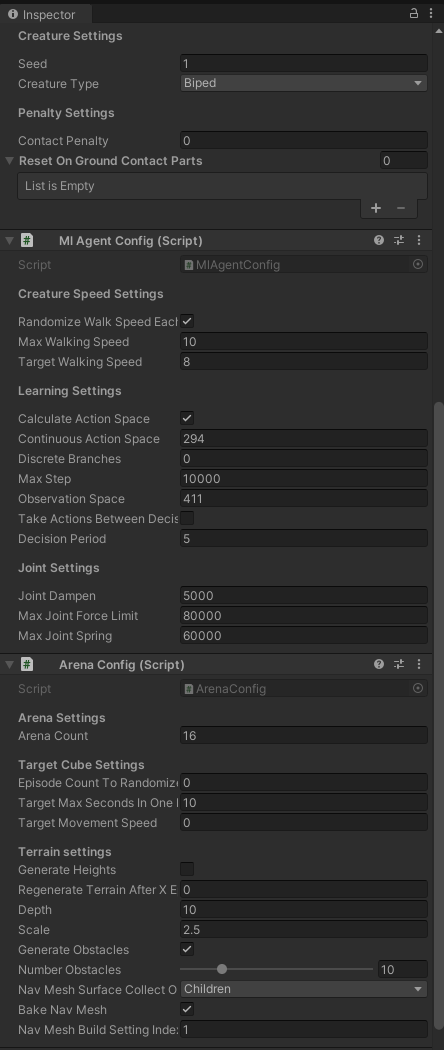
\includegraphics[width=0.4\linewidth]{resources/img/DEGConfig}
	\caption[Konfigurationsmöglichkeiten des \texttt{DynamicEnviormentGenerator}]{Konfigurationsmöglichkeiten des \texttt{DynamicEnviormentGenerator} im Unity-Editor.} 
	\label{bspDEGOptionen}
\end{figure}

\subsubsection{Aktuelle Version -- Advanced Environment Generator}
\begin{figure}
	\centering
	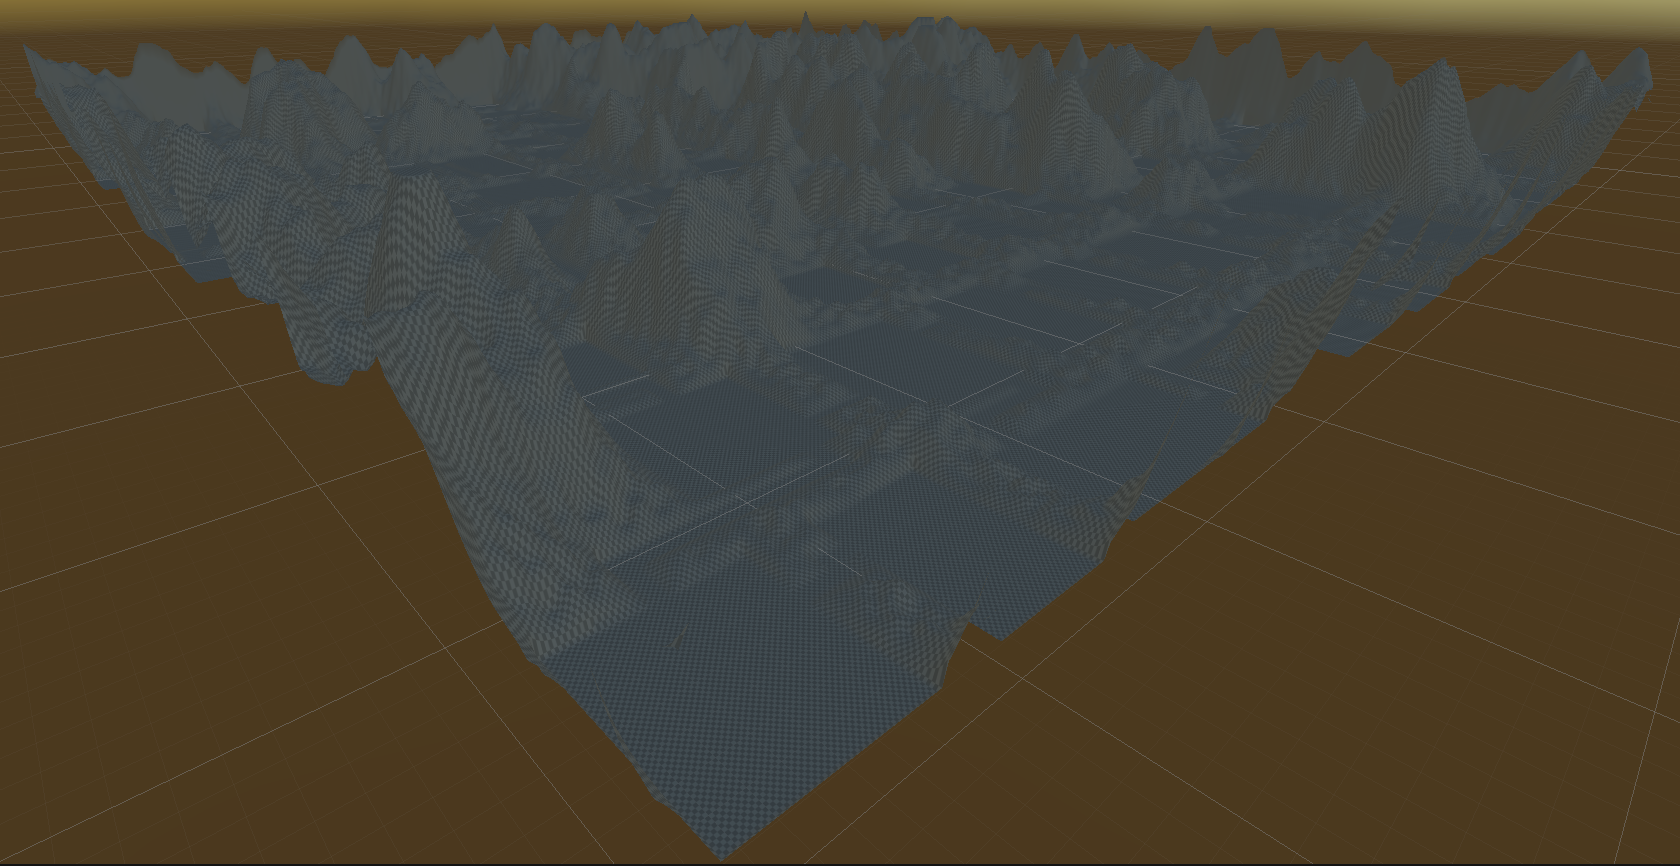
\includegraphics[width=0.7\linewidth]{resources/img/AEGArena.png}
	\caption[Konfigurationsmöglichkeiten des \texttt{AdvancedEnviormentGenerator}]{Ansicht der generierten Arena durch den \texttt{AdvancedEnviormentGenerator}.} 
	\label{bspAEGArena}
\end{figure}

Über den Produktzyklus des \texttt{DynamicEnviormentGenerator} sind insbesondere gegen Ende der Projektgruppe mehre Probleme aufgefallen. Da durch häufige Updates die Codequalität nachlässt und einige zuvor bedachte Optionen durch Zeitmangel nicht mehr relevant waren wurde entschieden, die Umgebung durch eine neue zu ersetzen. Dabei wurde insbesondere auf eine starke nähe zum Spiel geachtet, damit nur wenige Modifikationen für dieses erstellt werden müssen.

Die neue Umgebung wird im folgenden als \texttt{AdvancedEnviormentGenerator} bezeichnet und befindet sich in einer neuen Szene mit den Namen \enquote{AdvancedMovementScene}. Bedingt durch die konzeptionelle Weiterentwicklung der vorherigen Versionen mussten in den restlichen Skripten kaum Anpassungen durchgeführt werden. Eine Hauptänderung ist der geringeren Anzahl an verweisen auf den neuen Generator. Da der \texttt{DynamicEnviormentGenerator} in seinen ersten Versionen eine Art Gottklasse war, verwiesen die meisten andere Skripte darauf. Dies führte schnell zu unübersichtlichen Abhängigkeiten.

Die Generator-Klasse selbst konnte deutlich gekürzt werden, da eine Generierung von Arenen nicht mehr benötigt wird. Zu dem Zeitpunkt der Erstellung existierte bereits der \texttt{TerrainGenerator} für das finale Spiel, welche ab dieser Version für die Trainingsumgebung verwendet wird. Weiterhin ermöglichte dies eine Entfernung von vielen Einstellungen für das Terrain aus dem Generator-Objekt.

In der Abbildung \ref{bspAEGArena} ist das Endergebnis des \texttt{AdvancedEnviormentGenerator} dargestellt. Da es im realen Spiel zu Kollisionen zwischen verschiedenen Kreaturen kommen kann, wurde für die Trainingsumgebung nur eine zusammenhängende Arena verwendet. Insgesamt stimmen die Bedingungen für das Lernen und dem Spiel somit überein, da wie im Spiel kleine Korridore und Arenen mit ggf. mehreren Kreaturen genutzt werden.
\subsection{Erweiterung der Agent-Klasse}
\todo{texttt im Titel?}

\begin{figure}
	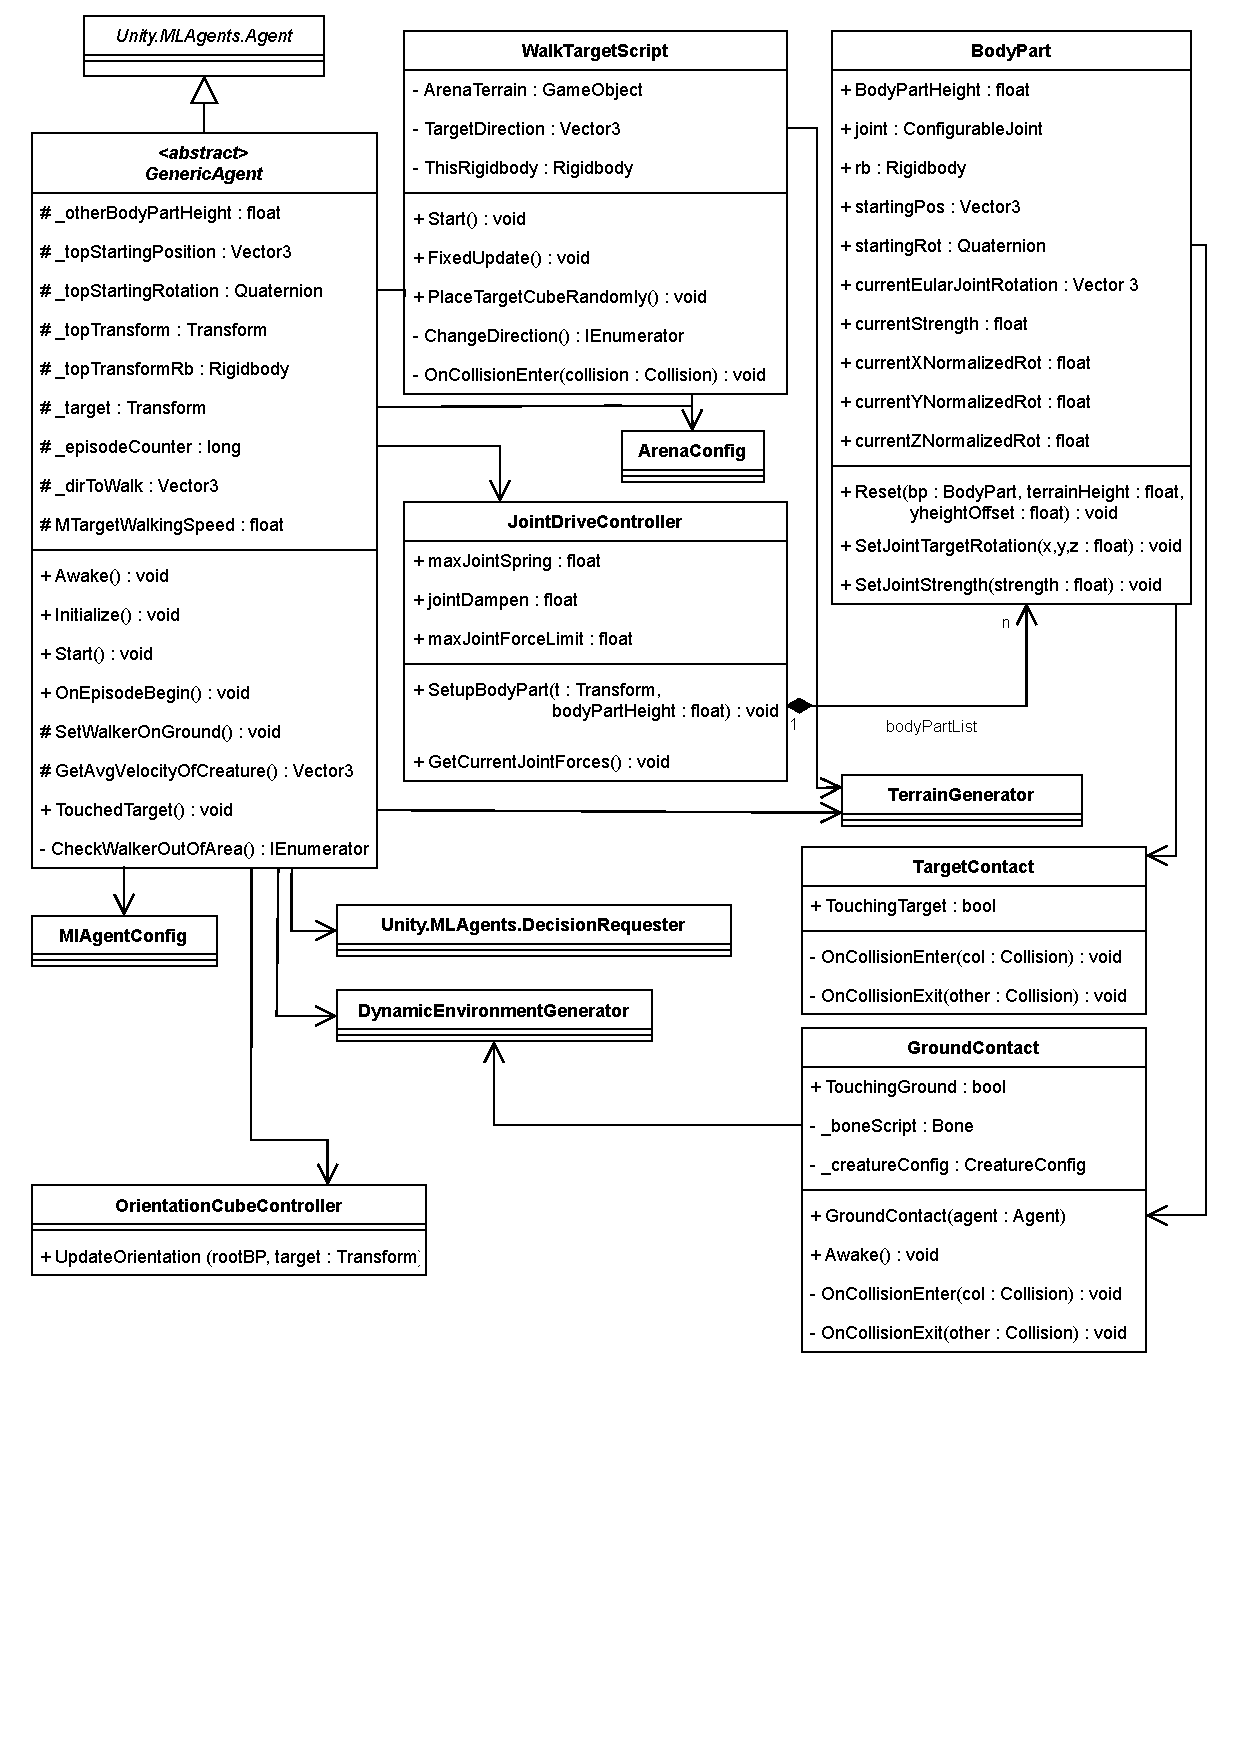
\includegraphics[width=\textwidth, trim={0cm 6.5cm 0cm 0cm}, clip]{resources/img/PG_Agent.drawio.pdf}
	\caption{UML-Diagram der GenericAgent-Klasse und weitere relevante Klassen}
	\label{fig:umlAgent}
\end{figure}

Als eine Erweiterung der \texttt{Agent}-Klasse von ML-Agents stellt die \texttt{GenericAgent}-Klasse das Verbindungsst"uck zwischen dem ML-Framework und der Unity-Engine dar. Im Folgenden wird der Aufbau der Klasse \texttt{GenericAgent} sowie derer Hilfsklassen \texttt{JointDrive\-Controller}, \texttt{BodyPart}, \texttt{OrientationCubeController} und \texttt{WalkTargetScript} erläutert und die Funktionalität dieser Klassen erklärt. Zur Veranschaulichung befindet sich in Abbildung \ref{fig:umlAgent} ein UML-Diagram. Der Aufbau dieser Klassen orientiert sich dabei sehr stark an die Implementierung des ML-Agents Walker.

\subsubsection{GenericAgent}

Die kontrollende Instanz einer konkreten Trainingsumgebung ist die \texttt{GenericAgent}-Klasse. Diese ist dazu in der Lage, mit dem Modell des ML-Frameworks zu interagieren, also sowohl Beobachtungen der Trainingsumgebung weiterzugeben also auch die Ausgaben des Modells anzunehmen (und zu verarbeiten). Außerdem ist die Klasse f"ur die Instandhaltung der Trainingsumgebung verantwortlich, indem sie Events der Umgebung verarbeitet (z.B. das Erreichen des Targets oder das Verlassen des zugänglichen Bereiches) und ggf. spezifizierte Routinen wie das Zur"ucksetzen der Umgebung durf"uhrt.
Schließlich muss die \texttt{GenericAgent}-Klasse noch die Rewards f"ur die Trainingsumgebung verteilen. Zu diesem Zweck ist die Klasse als \textit{abstract} definiert, da diese Rewardfunktionen stark von der Aufgabe des Agents abhängig sind. So benötigt zum Beispiel ein Agent, welcher ein bestimmtest Ziel möglichst schnell erreichen soll eine andere Reward-Funktion als ein Agent, welcher sich möglichst gut vor dem Spieler verstecken soll. Verschiedene Agents können so ohne Redundanz einfach als eine Erweiterung der \texttt{GenericAgent}-Klasse implementiert werden.

\todo{Mehr auf Reward-Funktionen eingehen oder erst bei konkreten Agents?}

\subsubsection{JointDriveController und BodyPart}

Um die Ingame-Repräsentation (also die generierte Creature) des Agents zu kontrollieren, besitzt der \texttt{GenericAgent} einen \texttt{JointDriveController}. Bei der Initialisierung der Trainingsumgebung wrappt der \texttt{JointDriveController} die verschiedenen Unity-Transforms der Creature in Instanzen der Hilfsklasse \texttt{BodyPart}. Die Klasse \texttt{BodyPart} gibt uns leichten Zugang zu häufig benötigten Funktionalitäten, wie zum Beispiel das Zur"ucksetzen oder Steuern des Transform. Auch besitzt ein \texttt{BodyPart} n"utzliche Informationen "uber das jeweilige Transform, welche dem ML-Modell weitergegeben werden können. Nach der Initialisierung stellt der \texttt{JointDriveController} nur noch das Verbindungsst"uck zwischen der \texttt{GenericAgent}-Klasse und der verschiedenen \texttt{BodyPart}-Instanzen dar.


\subsubsection{OrientationCubeController}

Da sich das Target des Agenten potentiell "uberall innerhalb einer großen (und weitgehend unbekannten) Ingame-Umgebung befinden kann, ist es hilfreich, die gezielte Laufrichtung des Agenten an eine einheitliche Position zu platzieren. Hierf"ur besitzt jeder Agent einen sogenannten \textit{OrientationCube}, welcher an einer festen Position relativ zum Agenten steht und sich lediglich in die Richtung des Targets dreht. So kann der Agent (und infolgedessen das ML-Modell) einfach den OrientationCube referenzieren, um die Laufrichtung zu bestimmen. Der \texttt{OrientationCubeController} stellt daf"ur die Reorientierungsfunktion des OrientationCubes bereit.


\subsubsection{WalkTargetScript}

Größtenteils unabhängig vom Agenten agiert das Target mithilfe des \texttt{WalkTargetScript}. Die Hauptaufgabe des Scripts ist es, das Target zu steuern (sowohl Neuplatzierung bei einem Reset, als auch normale Bewegungen innerhalb einer Episode) und beim Eintreten eines CollisionEvents zwischen dem Target und dem Agenten den Agenten zu notifizieren. Da zurzeit das Target nur aus einer Kugel besteht, ist komplizierteres Verhalten nicht notwendig.

\subsection{RL-Framework}
% Jannik

\subsubsection{Vorstellung des Frameworks}
Zum Trainieren der Kreaturen wird ein RL-Framework verwendet, welches mit den für die Kreaturen defininerten Agenten interagiert. Da das Projekt in Unity gebaut wird, stehen verschiedene Frameworks zur Verfügung, die sich in implementierten Algorithmen und Traininsoptionen unterscheiden. Da sich zu Beginn des Projekt bereits auf die Verwendung des Proximal Policy Optimization (PPO) Algorithmus geeinigt wurde, sind zwei Frameworks in der engeren Auswahl gekommen.

\paragraph{ml-Agents}\fup \label{mlAgentsFramework}
Das Unity Machine Learning Agents Toolkit \cite{juliani2020}, kurz ml-Agents, ist ein von Unity entwickeltes Projekt zum Trainineren von  und stellt, wie in diesem Projekt benötigt, unter anderem eine Implementierungen von PPO zur Verfügung.
Zusätzlich definiert das Toolkit auch eine Python API, die verwendet werden kann um eigene Agenten mit den zur Verfügung gestellten Algorithmen trainieren zu lassen.
Dabei unterstützt die API neben Diskreten und Kontinuierliche Aktions- und Beobachtungsräumne auch das Platzieren mehreren Agenten in einer Unity Szene.\\

\noindent Während der Trainigs angelegte Checkpoints und der finale Zustand des Netzwerks werden als onnx Dateien gespeichert, die dann geladen werden können, um das trainierte Netzwerk zu verwenden.\\
Zum Analysieren und Bewerten des Trainings erhebt ml-Agents verschiedene Daten, wie den durchschnittlichen Reward und die Loss Werte der verschiedenen Netzwerke und speichert diese in einem Tensorboard. 

\paragraph{neroRL}\fup \label{neroRLFramework}
Bei neroRL \cite{neroRL} handelt es sich um ein Reinforment Learning Framework, dass seinen Fokus auf verschiedene Varianten des Proximal Policy Optimization (PPO) Algorithmuses legt.\\
Der Agent kann dabei entweder mit geteilten oder getrennten Netzwerken und Gradienten für den Aktor und den Kritiker trainiert werden. \\
Dabei unterstützt es zum Trainieren neben openAIGym Umgebungen auch solche, die mit der Python API von ml-Agents erstellt wurden.\\
Die Observationsräume in diesem Umgebungen dürfen jedoch nur Vektor und Visuelle Beobachtungen enthalten und für die Aktionräume werden nur Diskrete und Multidiskrete Formate unterstützt.
Des weiteren kann in jeder Szene nur ein Agent platziert werden und zur Beschleunigung des Trainings müssen stattdessen mehrere Instanzen der Szene gleichzeitig trainiert werden.\\

\noindent Während der Trainings angelegte Checkpoints und der finale Zustand des Netzwerks werden als als pt Dateien abgespeichert und können als solche nicht direkt in eine Unity Umgebung geladen werden.\\
Zum Analysieren und Bewerten erhebt neroRL während des Trainings verschiedene Kenndaten, wie den durchschnittlichen Reward und die Loss Werte der verschiedenen Netzwerke und speichert diese in einem Tensorboard.

\subsubsection{Auswahl des Frameworks}

Beide vorgestellten Frameworks verfügen im Hinblick auf dieses Projekt über Vor- und Nachteile.

\paragraph{ml-Agents}\fup
ml-Agents unterstützt bereits von sich aus kontinuierliche Aktionsräume, welche zum Bewegen der Kreaturen benötigt werden. Außerdem erlaubt es mehrere Agenten in einer Szene zu platzieren, im folgenden als Multi-Agent-Szene bezeichnet, und so das Trainieren zu beschleunigen. 
Die vorherigen Tests mit der Walker Testumgebung in Unity \cite{walkerEnv} haben gezeigt, dass selbst eine zum Laufen optimierte zweibeinige Kreatur recht lange braucht, bis sie stabil und ohne umfallen laufen kann.
Bei einer prozedural generierten Kreatur ist zu erwarten, dass der Prozess länger dauert und darum sollten alle Möglichkeiten das Training zu beschleunigen verwendet werden.
Ein Problem mit ml-Agents liegt in der Auswertung von den Ergebnisse der Projektgruppe. Im Rahmen dieser Ausarbeitung ist es notwendig sich kritisch mit den Ergebnissen auseinander zu setzten und für den Teil der CreatureAnimation sind vor allem die Statistiken des Trainings relevant. Ml-Agents erhebt zwar im Rahmen des Trainingsvorgangs Statistiken und speichert diese in einem Tensorboard ab, allerdings werden nur wenige Statistiken erhoben. Zusätzlich speichert das Framework nicht direkt die erhobenen Werte ab, sondern in jedem Schritt nur den Durchschnitt der Werte. Für eine Analyse würde dies bedeuten, dass die verwendeten Daten bereits Durchschnitte sind und daher am Ende der Durchschnitt des Durchschnittes betrachtet wird, was keine guten Ergebnisse liefert. 
Ein weiterer Punkt ist, dass in der Konfiguration von ml-Agents eine maximale Anzahl von Checkpoints angegeben werden muss. Sollten im Laufe des Trainings mehr angelegt werden als dieses Limit erlaubt, überschreibt das Programm stattdessen die ältesten.
Der im Zweifel wichtigste Nachteil von ml-Agents ist jedoch, dass es sich bei dem Toolkit um ein sehr großes Projekt handelt, welches aus vielen einzelnen Modulen besteht. Aufgrund der Komplexität des Projekts wäre es sehr schwierig die zuvor genannten Nachteile zu beseitigen und es so an die Bedürfnisse der Projektgruppe anzupassen.\\
\paragraph{neroRL}\fup
Die Vorteile von neroRL sind zum einen, dass es mehr Informationen in das Tensorboard schreibt und die direkten Werte dort einträgt, ohne diese vorher zu verarbeiten. Außerdem verlangt die neroRL Konfiguration nur den Abstand zwischen Checkpoints und legt dann so viele Checkpoints an, wie nötigt. Im Kontrast zu ml-Agents werden gibt es keine maximale Anzahl und somit werden keine Checkpoints überschrieben. 
Zudem bietet neroRL eine Auswertungsfunktion, die nach dem Ende des Trainings verwendet werden kann, um bessere Daten zum Verlauf des Trainings zu erhaleten.
Dabei wird jeder angelegten Checkpoint des Netzes für eine festgelegte Anzahl an Episoden zu verwenden, um den Verlauf des Trainings und die Qualitätsunterschiede zwischen den Checkpoints darzustellen.
Die Nachteile von neroRL sind, dass nur Diskrete und Multidiskrete Aktionsräume unterstütze werden, welche zum Animieren der Kreaturen, nach vorläufigen Tests, nicht ausreichen werden. Außerdem erlaubt es nicht mehrere Agenten in einer Szene zu platzieren, was besser skaliert als die von neroRL zur Verfügung gestellte Variante mehreren Instanzen der Szene parallel zu trainieren. Im folgenden wird jeweils eine zum Trainieren verwendete Instanz der Szene als Build bezeichnet, da dies der Unity Terminologie entspricht. Eine Instanz einer Multi-Agent Szene ist entsprechend ein Multi-Agent Build.\\
\noindent Es ist also eindeutig, dass, unabhängig davon welches Framework gewählt wird, dieses noch angepasst werden muss, bevor es verwendet im Projekt werden kann. Es wurde sich schließlich für das neroRL Framework entschieden. Dieses Framework auf kontinuierliche Aktionen und Umgebungen mit mehren Agenten zu erweitern erschien einfacher, als in ml-Agents das Anlegen der Statistiken und Checkpoints so zu ändern, dass es für die notwendigen Analysen geeignet ist. 
Ein weiterer Einfluss auf diese Entscheidung war, dass Marco Pleines, der Entwickler von neroRL, als Betreuer in der Projektgruppe mitwirkt. Bei Fragen oder Problemen während der Anpassung können also deutlich schneller Feedback und Hilfestellungen gegeben werden, als dies bei Fragen zu ml-Agents der Fall wäre.

\subsubsection{Anpassung an neroRL} \label{neroAnpassungKonzept}
Bevor neroRL zum Trainieren verwendet werden kann müssen zunächst die zuvor aufgezählten Probleme mit dem Framework beseitigt werden.\\

\paragraph{Kontinuierlichen Aktionsräumen} \fup
Zunächst muss die Implementierung so erweitert werden, dass sie auch Umgebungen mit kontinuierlichen Aktionsräumen unterstützt. 
Um die Implementierung so einfach und übersichtlich wie möglich zu halten, wurde entschieden in diesem Schritt die Optionen für Diskrete und Multi diskrete Aktionsräume komplett aus der Implementierung zu entfernen. Da im Rahmen dieser Projektgruppe nur kontinuierliche Aktionsräume benötigt werden, genügt auch ein Framework, welches nur diese unterstützt. Zum Umsetzten der kontinuierlichen Aktionsräume muss die Ausgabe des Aktor Netzwerkes angepasst werden und diese wird in der \texttt{ContinuousActionPolicy} Klasse definiert. Diese implementiert einen Head (Kopf) für das neuronale Netzwerk, der kontinuierliche Aktionen umsetzt. Für jede Aktion des zugrundeliegenden Aktionsraumes werden $\mu$ (der Mittelwert) und $\sigma$ (die Standardabweichung) gelernt. Daraus wird eine Normalverteilung generiert, aus der dann ein tatsächliches Aktionstupel gesamplet werden kann. Als Verteilung wird die \texttt{Normal} Implementierung einer Gaußschen Normalverteilung aus PyTorch verwendet.

\paragraph{Multi-Agent Builds} \fup
In dem nächsten Schritt muss die Implementierung so erweitert werden, dass neroRL auch Multi-Agent Szenen unterstützt und nicht das Trainieren mit nur parallele Builds.
Abhängig von den verfügbaren Rechenressourcen lassen sich höchstens 16 Builds parallel ausführen (LiDo3 cgpu01 Knoten mit 2 Intel Xeon E5-2640v4 und 2 NVIDIA Tesla K40). 
Es wurde entschieden, dass vorhandene Verhalten mit mehreren parallelen Builds zu erweitert, sodass es parallele Multi-Agent Builds unterstützt. 
Die resultierende Implementierung sollte also in der Lage sein besser zu Skalieren, da nicht nur die Anzahl der Agenten in jeder Szene erhöht werden kann, sondern auch die Anzahl an Instanzen der Szene die parallel zum Trainieren verwendet werden. Diese Steigerung an Effizienz sollte mehr als ausreichend sein, um den zeitlichen Overhead durch das verarbeiten mehrerer Agenten pro Umgebung auszugleichen.
Abbildung \ref{fig:multi-agent-builds} zeigt vier parallel ausgeführte Multi-Agent Builds des MLAgents Walker Projekts, die jeweils 10 Agenten beinhalten. Insgesamt können so mit 40 Agenten parallel Erfahrungen gesammelt werden.
\begin{figure}
	\centering
	\includegraphics[width=0.7\linewidth]{example-image-a}
	\caption{Parallel ausgeführte Multi-Agent Builds}
	\label{fig:multi-agent-builds}
\end{figure}
Das von neroRL implementierte Systeme verwendet zum Sammeln der Erfahrungen Buffer, die ermöglichen jede Erfahrung genau ihrem  Build und dem Timestep an dem sie erstellt wurden zuzuordnen. 
Die Buffer mussten also erweitert werden, um zwischen den verschiedenen Agenten in einem Build zu unterscheiden, damit die Erfahrungen weiterhin zugeordnet werden können. 
Nach diesen Anpassungen hatten die Buffer die Dimensionen $[worker][agent][timestep][content]$. Über $[worker]$ und $[agent]$ werden alle Daten genau einem Agenten in einem der ausgeführten Builds zugeordnet. Für die $[timestep]$ Dimension wird außerdem für jeden Build und Agenten festgehalten, welches der aktuelle Zeitschritt ist. Da Umgebungen zu unterschiedlichen Zeitpunkten terminieren und zurückgesetzt werden, ist es möglich, dass die Zeitschritte zwischen verschiedenen Agenten nicht synchronisiert sind. Sobald genug Daten für die definierte Batchgröße gesammelt wurden, werden diese von den verschiedenen Builds und Agenten eingesammelt und in einem Batch kombiniert, welcher dann an den Trainingsalgorithmus übergeben wird.

\paragraph{Optimierung der Trainingsqualität} \fup
In einem letzten Schritt muss noch die Implementierung und Optimierung des verwendeten PPO Algorithmus betrachtet werden. Die aktuelle Implementierung ist für Diskrete Aktionen bestimmt und das Netzwerk kann daher nur aus einer stark begrenzten Anzahl an Aktionen auswählen. Bei einem kontinuierlichen Raum der für die Aktionen nur eine Ober- und Untergrenze festlegt gibt es deutlich mehr mögliche Aktionen. Daher kann es sein, dass die aktuelle Implementierung von PPO nicht genügt, um nach dem Training zufriedenstellende Ergebnisse zu liefern. Erste Tests belegten diese Befürchtung und lieferten unzureichende Ergebnisse. Beim Training der ml-Agent Walker Umgebung mit ml-Agents wurde nach ca. 30 Millionen Schritten einen durchschnittlichen Reward von ca. 2000 erreicht. Nach einem Test dieser Umgebung mit neroRL wurde auch nach über 150 Millionen Schritten nur einen Reward von ca. 220 erreicht.
Eine qualitative visuelle Bewertung des gelernten Verhaltens zeigt, dass der Walker sich zwar gezielt auf die erste Position des Ziels zubewegt, allerdings nach dem Verschieben des Ziels nicht in der Lage ist, sich umzudrehen. 
Um die Qualität des Trainings mit neroRL zu steigern, wurden verschiedene Optimierungen implementiert:

\begin{itemize}
	\item \textbf{Normalisierung der Observationen:} Die Observationen werden durch den Sampler automatisch normalisiert, um das Training zu stabiliseren und vor ausreißenden Werten zu schützen.
	\item \textbf{Squashing:} Grundsätzlich können die aus dem Netzwerk gesampleten kontinuierlichen Aktionen im Intervall $[-\infty;\infty]$ liegen. Auf Unity liegen die Aktionen im Intervall $[-1;1]$ und werden dementsprechend abgeschnitten. In einigen Fällen hat sich Tanh-Squashing als eine Methode erwiesen, um die Trainingsqualität mit kontinuierlichen Aktionen zu steigern und die Aktionen auf das Intervall $[-1;1]$ zu projizieren, anstatt diese abzuschneiden (vgl. \cite{shengyi2022the37implementation}). Unsere Implementierung von Tanh-Squashing wurde jedoch verworfen, da diese konsistent das Exploding-Gradients-Problem ausgelöst hat und das Training somit fehlgeschlagen ist. 
\end{itemize}

\subsection{LiDO3}
% Nils
Für die Trainingsdurchläufe wird das HPC-Cluster der TU-Dortmund genutzt. Zuänge hierfür wurden von unseren Projektgruppenbetreuern zur Verfügung gestellt. Um auf LiDO3 zu arbeiten wird mithilfe eines Gatewayservers auf das Cluster zugegriffen. Der Zugriff ist ausschließlich über das TU Dortmund Netzwerk möglich. Über den Gatewayserver kann ein Zugriff auf die Rechenressourcen direkt über die Shell oder über Skripte angefordert werden. Da die Shell-Methode einen dauerhaften Login erfordern würde, wird mit Skripten gearbeitet. Diese bestehen aus Konfigurationen für LiDO3 und den eigentlich Programmteil, welcher ausgeführt werden soll. LiDO3 nutzt als Jobmanager Slurm, weshalb die Skripte die Slurm-Syntax nutzen. Eine ausführliche Beschreibung die LiDO3 Konfiguration findet sich im Benutzerhandbuch\cite{lido};
\begin{listing}
	\begin{minted}[linenos,tabsize=2,breaklines]{shell}
#!/bin/bash -l
#SBATCH -C cgpu01
#SBATCH -c 20
#SBATCH --mem=40G
#SBATCH --gres=gpu:2
#SBATCH --partition=long
#SBATCH --time=48:00:00
#SBATCH --job-name=pg_k40
#SBATCH --output=/work/USER/log/log_%A.log
#SBATCH --signal=B:SIGQUIT@120
#SBATCH --mail-user=OUR_MAIL@tu-dortmund.de
#SBATCH --mail-type=ALL
#-------------------------------------
GAME_NAME="GAME_NAME"
GAME_PATH="/work/USER/games/$GAME_NAME"
module purge
module load nvidia/cuda/11.1.1
source /work/USER/anaconda3/bin/activate
conda activate /work/mmarplei/grudelpg649/k40_env
chmod -R 771 $GAME_PATH
cd $GAME_PATH
srun mlagents-learn /work/smnidunk/games/config/Walker.yaml --run-id=$GAME_NAME --env=t.x86_64 --num-envs=6 --no-graphics
	\end{minted}
	\caption{Skript zur Ausführung von ML-Agents auf LIDO3.}
	\label{prog:lidoSkript}
\end{listing}

In dem Beispielskript \ref{prog:lidoSkript} sind Anweisungen an die LiDO-Umgebung jeweils mit einem Kommentarzeichen gefolgt von \emph{SBATCH} gekennzeichnet. Die Konfiguration wird so gewählt, dass eine maximale Laufzeit mit exklusiven Ressourcenrechten auf den Rechenknoten besteht. Zusätzlich muss sichergestellt werden, dass eine Grafikkarte zur Verfügung steht. Diese stehen auf den \emph{cgpu01}-Rechenknoten mit jeweils 20 CPU-Kernen und 48 Gigabyte RAM zur Verfügung. Die maximale Laufzeit des Prozesses ist bei den GPU-Knoten auf \emph{long} begrenzt, was 48 Stunden entspricht. Es wird jeweils ein Log mitgeschrieben, aus dem der Trainingsfortschritt gelesen werden kann und bei besonderen Ereignissen eine Mail geschickt, um sofort benachrichtigt zu werden, falls der Job fertig ist oder fehlschlägt.

\subsubsection{Kompatibilitätsprobleme}
Um das beschriebene Skript auszuführen, muss auf LiDO3 eine ML-Agents-Umgebung installiert werden. Dabei handelt es sich um ein Python Umgebung, mit PyTorch und CUDA. In dem Slurm-Skript \ref{prog:lidoUmgebung} ist die Einrichtung einer funktionierenden Umgebung dargestellt. 

\begin{listing}
	\begin{minted}[linenos,tabsize=2,breaklines]{shell}
module purge
module load nvidia/cuda/11.1.1
source <anaconda3-path>/bin/activate
conda activate <env_to_install>
conda install torchvision torchaudio cudatoolkit=11.1 -c pytorch
python -m pip install mlagents==0.29.0 --force-reinstall
python -m pip install /work/mmarplei/grudelpg649/torch-1.10.0a0+git3c15822-cp39-cp39-linux_x86_64.whl --no-deps --force-reinstall 
	\end{minted}
	\caption{Installationsskript für Python und ML-Agents auf LIDO3.}
	\label{prog:lidoUmgebung}
\end{listing}

Für die Python-Installation wurde auf Anaconda\footnote{https://www.anaconda.com/} zurückgegriffen. Die installierte Anaconda-Arbeitsumgebung kann für die folgenden Schritte genutzt werden, indem die Slurm-Skripte diese am Anfang laden. CUDA kann als Kernelmodul in verschiedenen Versionen geladen werden oder per Anaconda installiert werden.

Problematisch ist die Installation von PyTorch, da ab Version 1.5 die Installationsbinärdateien keine Unterstützung für die von LiDO3 genutzten NVIDIA Tesla K40 Grafikarten bietet. Es besteht die Möglichkeit PyTorch zu bauen um die Unterstürzung zu erhalten. Dies musste für unsere Arbeitsumgebung nicht gemacht werden, da die PG-Betreuer ein Paket mit einer für LiDO funktionierenden PyTorch-Version von einer vorherigen PG zur Verfügung stellen konnten. Wie in \ref{prog:lidoUmgebung} dargestellt müssen zuerst die Abhängigkeiten von PyTorch, dann ML-Agents und zuletzt die spezielle PyTorch Version installiert werden, da sonst die Abhängigkeiten Probleme bereiten.

\subsubsection{NeroRL-Anpassungen}
\begin{listing}
	\begin{minted}[linenos,tabsize=2,breaklines]{shell}
GAME_NAME="GameMNSNero"
GAME_PATH="/work/<Username>/games/$GAME_NAME"
module purge
module load nvidia/cuda/11.1.1
module load gcc/11.1.0
source /work/<Username>/anaconda3/bin/activate
conda activate /work/mmarplei/grudelpg649/Jannik/neroEnv
chmod -R 771 $GAME_PATH
cd /work/<Username>/neroRL  
srun python -m neroRL.train --config /work/<Username>/games/config/Nero.yaml --run-id Generated2B --worker-id=6780 --env=$GAME_PATH/t
	\end{minted}
	\caption{Änderung des ML-Agents-Skripts für die Ausführung von NeroRL.}
	\label{prog:neroRlChanges}
\end{listing}
Im späteren Verlauf der PG wurde die Umstellung auf NeroRL durchgeführt. Dies bedeutet auf LIDO3 nur geringe Anpassungen, mit den Erfahrungen von ML-Agents der Aufrufprozess möglichst vereinfacht werden konnte. Eine Anleitung für die Installation steht im Github-Wiki\footnote{https://github.com/PG649-3D-RPG/neroRL/wiki}, des für diese Projektgruppe genutzten Forks, zur Verfügung.




	
	\chapter{Vorläufige Ergebnisse}
Unterkapitel nach Erkenntnissen. Metrik nach der bewertet wird erörtern. Objektiv ohne Wertung der Ergebnisse.

\section{Diskussion}
\label{Diskussion}

Dieser Abschnitt diskutiert die zuvor beschriebenen Ergebnisse der Projektgruppe im Bezug zur initialen Zielsetzung \ref{Zielsetzung_und_Vorgehensweise}.

\paragraph{Die Generierung von Spielleveln}

\paragraph{Generierung der Monster}

\paragraph{Fortbewegung der Monster}
	
	\chapter{Ausblick}
\label{Ausblick}
	
	\chapter*{Themenallokation}

\begin{thallok}
	\item Einleitung: Thomas
	\item Grundlagen
	\begin{thallok}
		\item Reinforcement Learning: Jannik
		\item Cellular Automata: Markus
		\item L-Systeme: Kay
	\end{thallok}
	\item Verwandte Arbeiten
	\begin{thallok}
		\item RL Frameworks
		\begin{thallok}
			\item ML-Agents: Niklas
			\item NeroRL: Niklas
		\end{thallok}
	\end{thallok}
	\item Fachliches Vorgehen:
	\begin{thallok}
		\item Projektorganisation: Carsten, Thomas, Jannik, Leonard
		\item Creature Generation
		\begin{thallok}
			\item Metaballs: Jona
			\item Jonas Creature Generation Method: Jona, Markus
			\item L-System Creature Generation: Tom, Kay
			\item Mesh Generation: Leonard
			\item Automatisches Rigging: Leonard
		\end{thallok}
		\item Creature Animation
		\begin{thallok}
			\item Trainingsumgebung: Carsten
			\item Training: Niklas
		\end{thallok}
		\item Terraingeneration
		\begin{thallok}
			\item Dungeon Generierung: Tom
			\item Space Partitioning: Tom
			\item Perlin Noise (Terrain-Flächen): Kay
			\item \sout{Vegetation via L-System: Kay} für Endbericht, bisher nicht implementiert
		\end{thallok}
	\end{thallok}
	\item Technische Umsetzung
	\begin{thallok}
		\item Creature Generation: Markus
		\item Creature Animation: Nils, Carsten, Jan
		\begin{thallok}
			\item Trainingsumgebung: Nils
			\item Erweiterung der Agent Klasse
			\item LiDO3
			\item Training: Jannik
		\end{thallok}
	\end{thallok}
	\item Vorläufige Ergebnisse
	\begin{thallok}
		\item Diskussion
	\end{thallok}
	\item Ausblick
\end{thallok}


	
	\listoffigures				% Abbildungsverzeichnis ... nicht für kurze Dokumente
	\cleardoublepage
	\listoftables				% Tabellenverzeichnis
	\cleardoublepage
	\pagenumbering{arabic}
	\setcounter{page}{4}
	\cleardoublepage				
	% \bibliographystyle{IEEEtran}	% Das Literaturverzeichnis; ieeetran verwenden, damit auch URLs angezeigt werden
	% \bibliography{seminar-lit}
	\printbibliography
	
	
\end{document}